\chapter{Search for the $\hmumu$ decay}

\textit{"The Higgs boson may, or may not, couple to the second generation fermions."}

\vspace{5mm}
\begin{flushright}
--- a bright bunch of ATLAS scientists.
\end{flushright}

\thispagestyle{empty}
\newpage

The interactions between the Higgs boson and the vector bosons and
third generation fermions, critical to the discovery in 2012, soon 
became the preferred way to study the properties of the Higgs boson.
The mass \cite{Aad:2015zhl, Aaboud:2018wps, CMS-PAS-HIG-19-004},
as well as inclusive and differential cross-sections
\cite{Aad_2015, Chatrchyan_2014, Aaboud:2017oem, Sirunyan:2018sgc, Aaboud:2018ezd},
have been measured and new production modes, $\tth$ \cite{Sirunyan:2018hoz, Aaboud:2018urx}
and $\vh$ \cite{Sirunyan:2018kst, Aaboud:2018zhk}, have been 
observed. However, the interactions between the Higgs boson
and the first or second generation of fermions have not been
observed yet due to experimental challenges. In the leptonic
sector the main challenge is a very small branching fraction due
to the small mass of electron and the muon compared to the tau.
In the quark sector some branching ratios, for example to the charm
quark pair, are larger than those in which the Higgs was discovered.
However, detection is experimentally difficult in the LHC environment
due to the difficulty in flavour tagging, and estimating and modelling
backgrounds \cite{Aaboud:2018fhh, CMS-PAS-HIG-18-031}. Ultimately the
decay to muon pairs offers the best sensitivity to probe the
interactions between the Higgs boson and the second generation
fermions.

In the Standard Model the branching ratio of the Higgs boson with a
mass of 125.09 \GeV~is predicted to be $2.17 \times 10^{-4}$
\cite{deFlorian:2016spz}. This could be modified by physics beyond the
SM \cite{Giudice:2008uua, Dery:2013rta, PhysRevD.80.095023}, meaning
that any deviation from the predicted value could be a sign of new
physics.

ATLAS and CMS experiments have already conducted searches using
the LHC Run 1 data collected at centre-of-mass energies $\sqrts = 7$
and 8 \TeV, both setting the 95\% confidence level upper limits on the
product of the Higgs production cross-section and the branching ratio
to muon pairs \cite{Aad:2014xva, Khachatryan:2014aep} of about seven
times the SM expectation. Using the data collected at $\sqrts = 13$
\TeV, in years 2015 and 2016 the observed upper limit was further
decreased to 2.8 and 2.9 by ATLAS and CMS respectively
\cite{Aaboud:2017ojs, CMS-PAS-HIG-17-019}, with ATLAS
further updating its result to 2.1 using the data collected in 2017
\cite{ATLAS-CONF-2018-026}. This corresponds to $0.9 \sigma$ expected
significance, meaning that the channel is on the verge of evidence.

This chapter presents the search for the Higgs boson decay to muon
pairs using full ATLAS Run 2 dataset collected between 2015 and 2018
at $\sqrts = 13$ \TeV, almost doubling the integrated luminosity of
the dataset since the last result to $139~\ifb$. The Higgs boson mass
is assumed to be 125.09 \GeV~for all presented results.

The overall strategy of the analysis is to select events with
two oppositely charged muons passing the single muon triggers,
and apply additional requirements
to reduce $\ttbar$ and diboson backgrounds. Events are then split
in three channels based on whether they contain zero, one, or two or
more jets in addition to the muon pair. They are further split in
individual categories using a multivariate discriminant, based
on the differences in kinematics between the muon pairs coming
from a Higgs boson produced in the main production modes, and the
muon pairs coming from background events, which are dominated by
the Drell-Yan spectrum. Signal events tend to be more central and
have higher transverse momentum, their jet multiplicity is higher,
and the VBF production mode has a unique signature of two 
back-to-back high-$\pt$ jets with little hadronic activity between
them. Finally, a maximum likelihood fit to the dimuon invariant mass
spectrum is performed in all categories simultaneously, extracting
the signal strength parameter. The analysis is limited by
statistical uncertainty arising from a limited size of the dataset.
The systematic uncertainties are dominated by the uncertainty on
the background modelling, assessed using a dedicated simulated sample.
Additional systematic uncertainties arise from the normalisation 
of signal sample and migration between the categories, such as
the uncertainty on the production cross-section and branching ratio
from the theoretical side, and luminosity, muon momentum resolution
and detector calibration from the experimental side.

A number of improvements were introduced with respect to the
previous result. Selection was improved by including additional
muons from the corners of detector acceptance, by improving
the resolution of the invariant mass by recovering the final
state radiation, and by better rejection of \pileup~ jets in the
forward region. The allocation of events in the categories was
improved by employing a fully multivariate approach in lieu
of a hybrid approach combining a multivariate discriminant and 
cut-based categories. Finally, the background modelling was
improved by using a new functional form and larger DY simulation
dataset. The total effect of all improvements is an approximately
20--30\% increase in the analysis sensitivity and is dominated
by the improvements from using a fully multivariate categorisation
approach.

\section{Data and MC simulation samples}

The proton-proton collision data used in this analysis was
collected in 2015, 2016, 2017, and 2018 at the centre-of-mass
energy of 13 \TeV~in the main physics stream. It corresponds
to an integrated luminosity of 139 $\ifb$ after passing the data
quality checks which ensure that the important parts of the
detector are switched on and function as intended.

The MC simulation samples are used in the analysis for a 
variety of purposes. The signal samples are used to optimise
the event selection and to determine the normalisation and
shape of the signal model in the analysis categories.
Centrally produced background MC simulation samples are used
to optimise the event selection and to validate the muon
momentum resolution in the analysis categories, but not to
determine the normalisation or shape of the backgrounds.
While the normalisation and shape parameters are determined
in the final fit to data, the functional form is selected
in each analysis category independently using a custom
high-statistics MC simulation of Drell-Yan events.

\subsection{Background samples}

\label{sec:bkg-mc}

The leading irreducible background for the analysis is the
Drell-Yan (DY) production of muon pairs. It is simulated using
\textsc{Sherpa} 2.2.1 with the NNPDF3.0 set of parton
distribution functions (PDF) \cite{Ball:2014uwa} in slices of
$\HT$ and with $c$- and $b$-quark filters, simulating 0--2
jet events at next-to-leading order (NLO) and at leading order
(LO) for 3 and 4 jets using \textsc{Comix} \cite{Gleisberg:2008fv}
and \textsc{OpenLoops} \cite{Cascioli:2011va, Denner:2016kdg}
libraries. Matching with the \textsc{Sherpa} parton showering
\cite{Schumann:2007mg} is done using the MEPS@NLO prescription
\cite{Catani:2001cc, Hoeche:2012yf, Hoeche:2011fd}.
In order to populate the tails of the
DY invariant mass distribution relevant for the analysis an
additional high-statistics sample is generated with identical
setup an an additional cut of $\mmumu > 100$ \GeV. Finally, 
\textsc{Sherpa} is also used to model the electroweak $Z$+jets
process with up to two additional jets at LO accuracy beyond
the first two jets.

With the mass of the top-quark set to $m_t = 172.5$ \GeV, the
$\ttbar$ and single-top samples are generated using
\textsc{Powheg-Box} \cite{powheg, Frixione_2007, Alioli_2010}
with NNPDF3.0 PDF set and parton showering and hadronisation
done in \textsc{Pythia} 8.186 using the A14 parameter set
\cite{ATL-PHYS-PUB-2014-021}. $\ttbar$ cross-section is
computed to next-to-next-to-leading order (NNLO) in
QCD with next-to-next-to-leading logarithmic
(NNLL) soft gluon terms taken into account. The cross-section
of the single-top is computed with prescriptions from
\cite{Kidonakis:2011wy, Kidonakis:2010ux}, and all the processes
($t$-channel, $s$-channel, and $Wt$-channel) are generated
separately.

Diboson processes, $WZ$ and $ZZ$, are generated using
\textsc{Sherpa} 2.2.1 with the NNPDF3.0 PDF set, and are normalised
directly to the \textsc{Sherpa} prediction. Only semi-leptonic
and fully-leptonic decays are simulated.

\subsection{Signal samples}

The largest contribution comes from the $\ggf$ signal sample,
generated with \textsc{Powheg-Box} with PDF4LHC15 PDF set
to next-to-next-to-leading order accuracy with parton shower matching
(NNLOPS) \cite{Hamilton:2013fea}, achieving NNLO in QCD after
the re-weighting in rapidity of the Higgs boson. The cross-section
for the $\ggf$ production mode are computed to
next-to-next-to-next-to-leading order (N3LO) \cite{Anastasiou:2016cez}
in QCD with NLO electroweak corrections applied
\cite{Aglietti:2004nj, Actis:2008ug} under the assumption that
they factorise. \textsc{Pythia} 8 with the AZNLO parameters
\cite{Aad:2014xaa} is used to simulate the decay
of the Higgs boson, final state photon radiation, parton
showering, and hadronisation. 

$\vbf$ and $q\bar{q}/qg \rightarrow \vh$ production modes are
generated to NLO accuracy in QCD using \textsc{Powheg-Box},
while the $gg \rightarrow ZH$ is generated to LO accuracy. Same
PDF set and \textsc{Pythia} tunes are used as in the $\ggf$
generation. VBF cross-section is computed with full NLO QCD
and electroweak corrections \cite{Ciccolini:2007jr, Ciccolini:2007ec,
Arnold:2008rz}, and approximate but highly accurate NNLO QCD
corrections \cite{Bolzoni:2010xr}. VH cross-section is computed at
NNLO in QCD \cite{Brein:2003wg} with NLO eletroweak
corrections \cite{Ciccolini:2003jy}, apart from the
$gg \rightarrow ZH$ which is computed to NLO and next-to-leading-logarithm
accuracy in QCD \cite{Ciccolini:2003jy, Brein:2003wg, Brein:2011vx,
Altenkamp:2012sx, Denner:2014cla, Brein:2012ne, Harlander:2014wda,
Harlander:2018yio}.

$\tth$ production mode is generated using \textsc{MadGraph5\_aMC@NLO}
\cite{Alwall:2014hca, Artoisenet:2012st} at NLO accuracy using
NNPDF3.0NLO PDF set and the A14 tune. The cross-section is
computed to NLO in QCD with NLO electroweak corrections
\cite{Yu:2014cka, Beenakker:2002nc}.

\textsc{Pythia} is also used to
overlay minimum bias events to model the effects of \pileup~for all
simulated events using the NNPDF2.3LO PDF set \cite{Ball:2012cx}
with the A3 parameters \cite{ATL-PHYS-PUB-2016-017}. All signal
and background samples are passed through the full ATLAS
detector simulation. Pile-up re-weighting, object momentum
smearing, and efficiency scale factors are applied to the MC
simulation samples in order to make them mimic the collected data.

\subsection{Custom Drell-Yan sample}
\label{sec:hmumu:customDY}

Extract the signal strength paramater relies on a
maximum likelihood fit to the invariant mass spectrum in data,
using parametrised models of both signal and background. The choice
of the functional form describing the background is crucial because
a mismodelling of the background results in a bias on the extracted
signal strength. This is particularly significant when the
signal-to-background ratio is very small, because the impact can be
large.

In order to select the functional form and evaluate the resulting
bias, referred to as the ``spurious signal", a fit to the
background-only spectrum is performed. Ideally, this would be done
on the background MC simulation described in Section \ref{sec:bkg-mc},
but because of the high computational cost associated with the 
simulation of the detector response the statistics of the sample
are on the same order of magnitude as the data. As a result, the
the extracted spurious signal value is unreliable and dominated by
the statistical fluctuations. A custom high-statistics sample of DY
events is generated to overcome this challenge.

The custom DY sample needs to have significantly larger statistics
than the data, requiring a much faster generation. To facilitate
this, the sample is produced at a generator-level only, skipping
the simulation of showering, hadronisation, and detector response,
replacing them by parametrised smearing functions. The effect on
the dimuon invariant mass spectrum is minimal, and because of the
parametrised smearing the jet mismodelling is a second order effect.
On the other hand, final state radiation (FSR) does have an effect on
the invariant mass spectrum and is simulated by \textsc{Photos++}
\cite{Golonka:2006tw}. This setup was fast enough to generate 20
billion events corresponding to approximately 100 $\iab$ in the 
regions of parameter space relevant for the analysis. A drawback of
the sample is that it only models the dominant DY part of the
invariant mass spectrum.

At generator level, the samples are produced separately for zero
or one parton and two partons in addition to the muon pair:
\begin{itemize}
\item \textsc{Powheg} is used to generate an inclusive NLO $\zmumu$
sample, modelling zero and one parton in addition to the muon pair.
For efficiency reasons two sub-samples are generated, one with
$60 < \mmumu < 95$ \GeV~($2.5\times10^{9}$ events), and the other
with $\mmumu > 95$ \GeV~($10\times10^{9}$ events) requirement. Even
after detector smearing the latter sample dominates the fit region.
\item \textsc{Alpgen} \cite{Mangano:2002ea} is used to generate
events with two partons in addition to the muon pair at LO. The 
computation uses only the matrix element with two additional
partons and requires both of them to have $\pt > 25$ \GeV~as well
as $\Delta R(j,j) > 0.4$ to minimise the overlap with the
\textsc{Powheg} sample. Similarly to the \textsc{Powheg} sample,
events are generated with $60 < \mmumu < 95$ \GeV~($1.75\times10^{9}$
events) and $\mmumu > 95$ \GeV~($2.5\times10^{9}$ events)
requirements. These events are crucial to populate the analysis
categories with a large fraction of the signal events coming from
the VBF production mode.
\end{itemize}
Both samples are corrected in the same way to model the effects of
the detector. Muon momentum smearing is done using parametrised functions
derived from MC simulation described in Section \ref{sec:bkg-mc}.
Effects from identification, reconstruction, isolation, and impact
parameter efficiencies are also derived from MC simulation and 
applied as weights, while trigger efficiency weights are derived
from data. FSR momentum is smeared using parametrised prescription
from the ATLAS subgroup specialising in electrons and photons.
Photons are dropped randomly to emulate the reconstruction
efficiency. Smearing of jet momenta is performed using the parametrisation
from the ATLAS subgroup specialising in jets and missing energy.
The effect of \pileup~jets is modelled by building a library of
jets from minimum-bias events in MC simulation and overlaying a
number of sampled jets from the library for each event. A dedicated
missing transverse energy ($\met$) smearing is derived from the Run 2 data.

\section{Physics objects}

The search for a narrow resonance on top of a smoothly falling
background appears at first sight to require not much more than an
excellent understanding of muons in ATLAS. While the intirety of Chapter
\ref{sec:muons} is dedicated to their performance, the sophistication
of the analysis requires understanding of other objects as well.
Photons are used to recover the final state radiation in order to improve
the resolution of the invariant mass spectrum. Jets are used
as a handle to select events produced in the VBF production mode
and to improve separation from the other backgrounds. Even electrons
are reconstructed, albeit solely in order to reject fake jets. Finally,
missing transverse energy is used to supress top and diboson
backgrounds.

\subsection{Muons}

Muon reconstruction, identification, and isolation are described in
detail in Chapter \ref{sec:muons}. Table \ref{tab:hmumu:muons}
summarises the selection used for the $\hmumu$ analysis.
\begin{table}[h]
\centering
\caption{Summary of the muon selection requirements.}
\label{tab:hmumu:muons}
\begin{tabular}{c c}
\toprule
\midrule
ID selection & Loose \\
\midrule
Isolation selection & FixedCutPflowLoose \\ 
\midrule
$\pt$  & $\pt > 15$ \GeV \\
\midrule
$\eta$ & $|\eta| < 2.7$ \\
\midrule
\multirow{2}{*}{Impact parameters} & $|d_0 / \sigma_{d_0}| < 3.0$ \\
                                   & $|z_0 \cdot \sin{\theta}| < 0.5$ mm\\
\midrule
\bottomrule
\end{tabular}
\end{table}
The majority of reconstructed muons in the Loose selection are
the CB type, combining the information from the tracker and
muon spectrometer systems. However, in order to maximise the
acceptance of signal events other muons types are also used
to improve the reconstruction efficiency in the challenging
parts of the detector. ST and CT improve the reconstruction
efficiency in the $|\eta| < 0.1$ region where the muon
spectrometer has a gap to allow for cabling and services to
the tracker, while the ME muons are used in the forward
regions to reconstruct muons outside of the tracker
coverage, where $2.5 < |\eta| < 2.7$.

CB muons benefit from a combination of two $\pt$ measurements,
the one in the tracker, and the one in the muon spectrometer.
Figure \ref{fig:hmumu:reso} verifies that the resulting dimuon
invariant mass resolution is only marginally worse for muon
pairs containing one non-CB muon (dotted green line) compared
to pairs where both muons are CB (dashed blue line). Since
most muons are CB, the inclusive distribution (solid orange
line) and the distribution of purely CB muons (dashed blue line)
are nearly identical.

The reason for such a small degradation is that the resolution of the combined
$\pt$ measurement is dominated by the tracker $\pt$ measurement
in the barrel region, and by the muon spectrometer measurement
in the forward regions. ST and CT muons, used in the $|\eta| <
0.1$ region, combine a track in the ID with a segment in the
muon spectrometer or with a calorimeter deposit, and thus 
benefit from having the high-quality tracker $\pt$ measurement.
Conversely, ME muons, used in the $2.5 < |\eta| < 2.7$ region,
use the track from the muon spectrometer, the higher quality
measurement in the forward region.
\begin{figure}[h!]
  \centering
  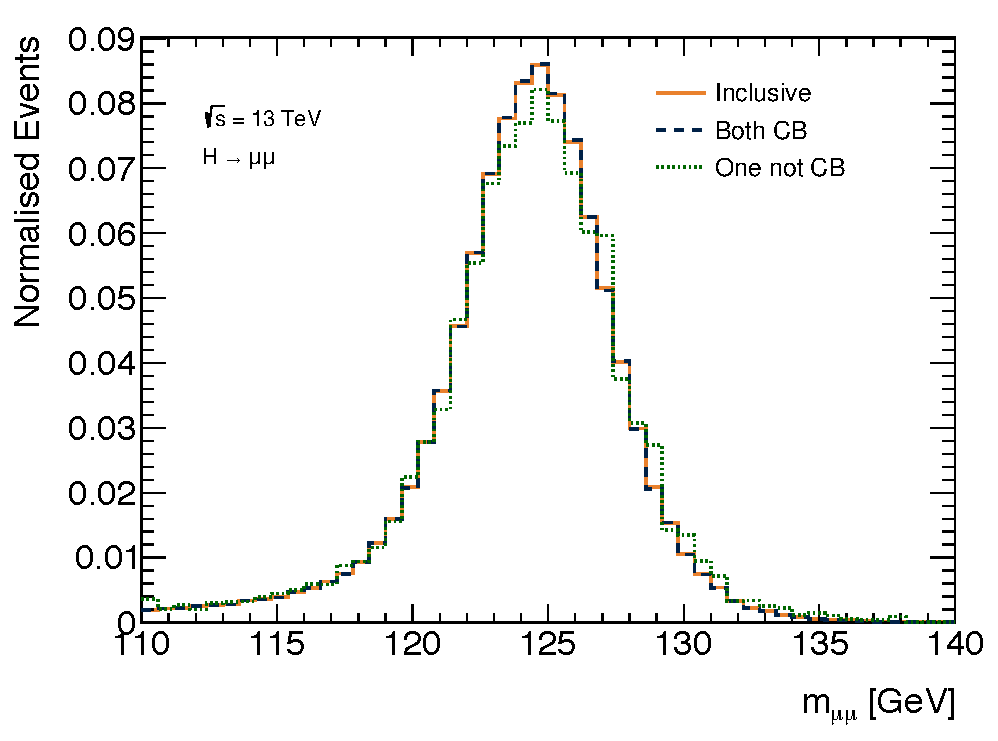
\includegraphics[width=0.8\textwidth]{figures/hmumu/resolution}
  \caption[Muon resolution for different muon types]{Resolution
  of the dimuon invariant mass measurement for the $\ggf$ signal
  sample in the $\hmumu$ analysis signal region. Events in which
  both muons are CB type are shown in dashed blue line, while
  events in which one of the muons is not CB are shown in dotted
  green line. Inclusive distribution is shown in the solid orange
  line.}
  \label{fig:hmumu:reso}
\end{figure}
The FixedCutPflowLoose isolation selection is used because
of a combination of its high efficiency, robustness to high
\pileup~conditions, and an improved rejection of heavy-flavour
jets. The cut on the $\pt$ rejects muons from the decay of
heavy-flavour quarks, while cosmic rays are rejected by the
standard requirements on the impact parameters.

\subsection{Photons and FSR}

Photons are reconstructed in ATLAS via its energy deposits
in the eletromagnetic calorimeter. Unlike electrons, photons
are electrically neutral and do not leave tracks in the
tracker, unless they are converted to electron-positron
pairs before reaching the calorimeter. The details on the
reconstruction algorithm and its performance are described
in Ref. \cite{Aaboud:2018yqu}.

Muons may radiate a photon and thus lose energy, meaning that
the invariant mass of the muon pair is no longer equal to the
mass of the mediator. In order to mitigate this effect up to
one final-state photon candidate is added to the mass
calculation, using a procedure similar to the one used in
Ref. \cite{Aad:2014eva}, but optimised for the high-purity
requirements of this analysis. Collinear photons
($\Delta R(\gamma, \mu) < 0.20$) are required to have $\pt$
larger than a linearly increasing threshold, from
$\pt^\gamma > 3$ \GeV~at $\Delta R(\gamma, \mu) = 0$ to
$\pt^\gamma > 8$ \GeV~at $\Delta R(\gamma, \mu) = 0.2$.
Non-collinear photons ($\Delta R(\gamma, \mu) > 0.20$)
are required to have $\pt^\gamma > 8$ \GeV~and tight \cite{Aaboud:2018yqu}
identification requirement for photons. When multiple
photon candidates are found only the one with the highest $\pt$
is included in the invariant mass calculation, with priority
to the collinear photons over non-collinear ones.

Around 5\% of all signal events have at least one FSR candidate,
of which approximately 90\% are the collinear photons.
The distribution of invariant mass for the MC simulation of
$\ggf$ signal events with at least one reconstructed FSR
candidate is shown in Figure \ref{fig:hmumu:fsr}
before and after the recovery of final state radiation.
It can be seen that the mass peak is shifted much closer to
125 \GeV, with the slight overshoot resulting from the fake
FSR candidates coming from pileup. The improvement in the
invariant mass resolution is approximately 3\% inclusively.
A drawback of the FSR recovery is an $\sim 8\%$ increase in the
number of background events in the signal region due to the
migration of events from the $Z$ mass peak.
\begin{figure}[h!]
  \centering
  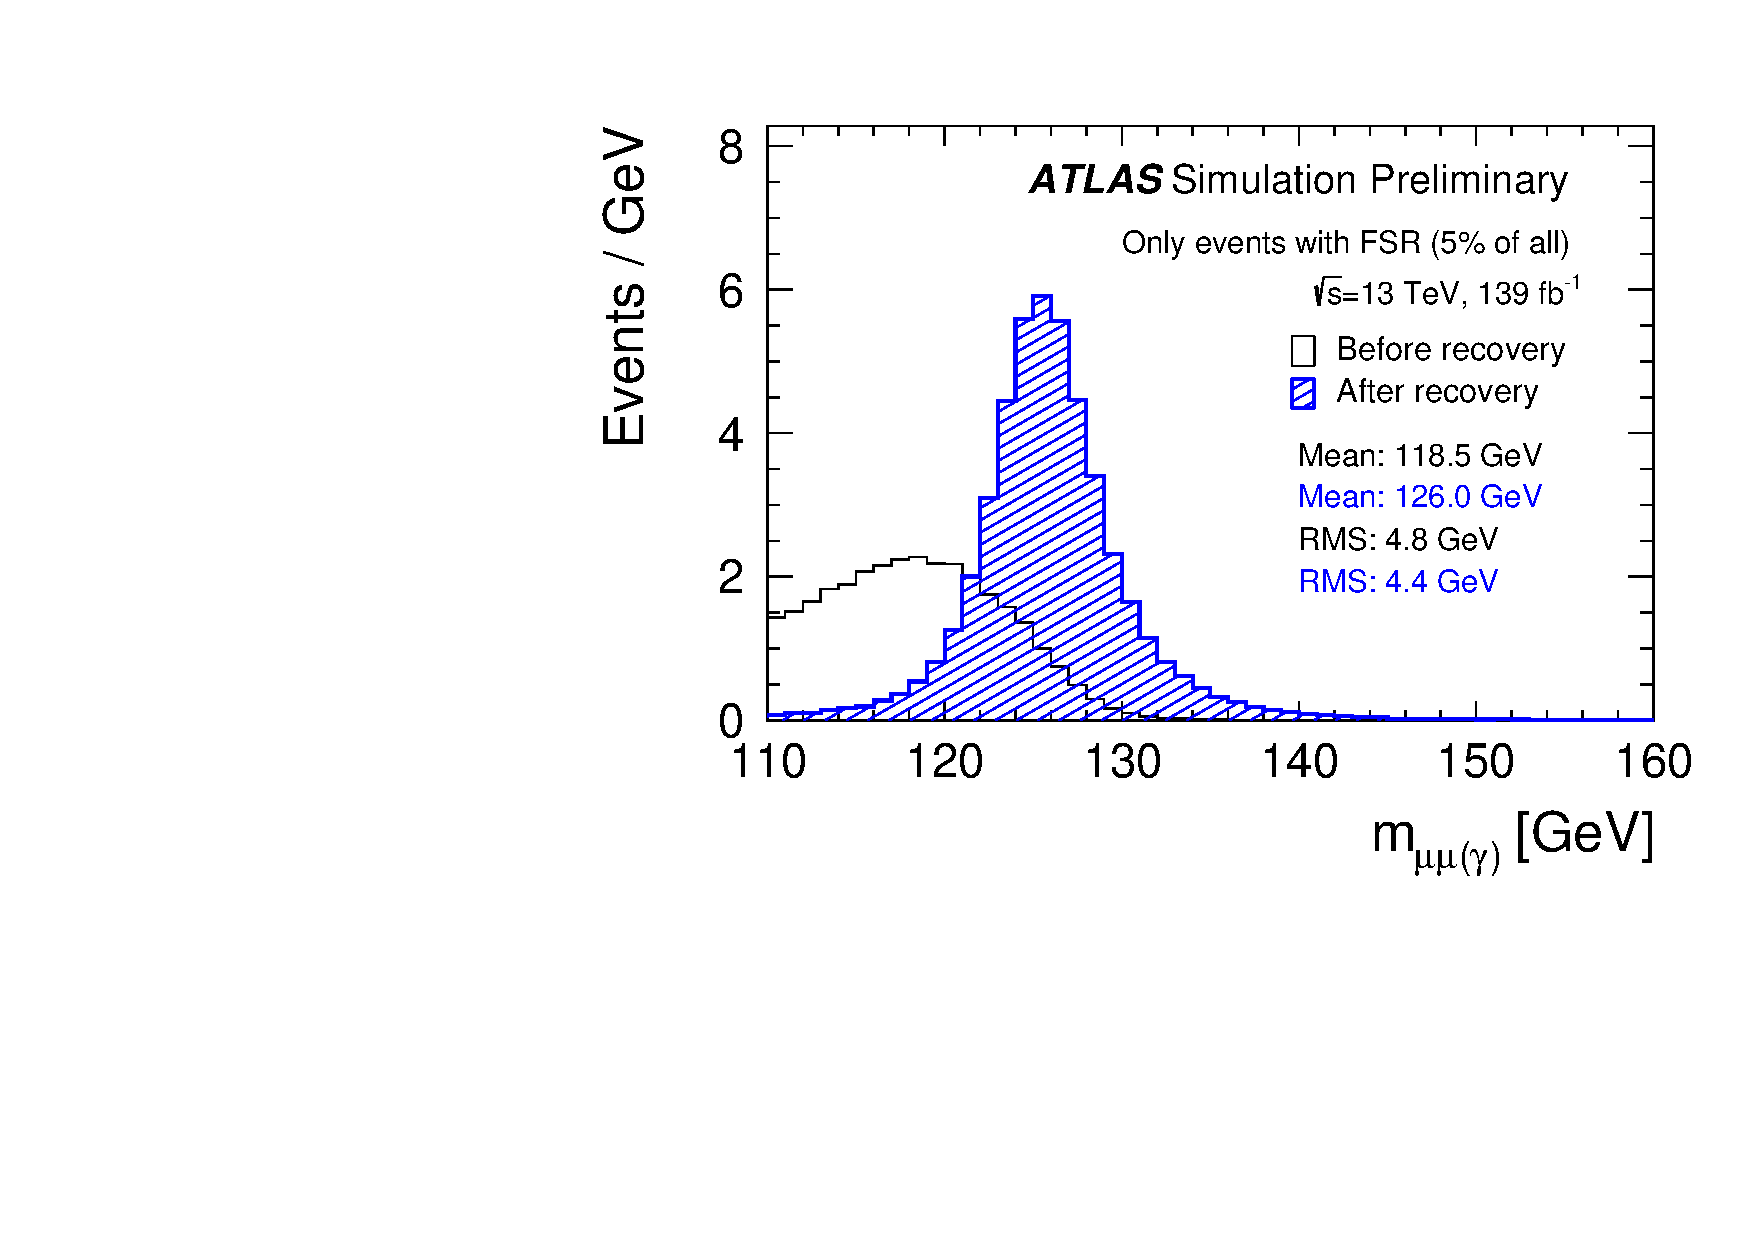
\includegraphics[width=0.8\textwidth]{figures/hmumu/FSR_fsr}
  \caption[Final state radiation recovery]{Invariant mass before
  (white solid) and after (blue hatches) final-state radiation
  recovery for a MC simulation of $\ggf$ signal events passing
  the analysis selection. Only events with one or more
  reconstructed FSR candidates are shown. The mean and the
  root-mean-square of the distributions are shown in the bottom
  right corner. From Ref. \cite{ATLAS-CONF-2019-028}.}
  \label{fig:hmumu:fsr}
\end{figure}

\subsection{Jets, electrons, and $\met$}

Jets are the collimated collections of hadrons, arising either
from a parton in the final state of the interaction, the remnants
of the proton not participating in the hard scatter (underlying event),
or from \pileup~interactions. They are used to identify events
which could have been produced via the VBF production mode by
exploiting its typical dijet signature. Jets are experimentally the richest
objects in ATLAS, reconstructed either from the deposits in the
calorimeters, tracks that the charged hadrons leave in the tracker,
or both. The optimal use of substructure has been extensively
studied both theoretically \cite{Altheimer:2012mn} and using
a wide variety of modern machine learning techniques \cite{Larkoski:2017jix}.
The reconstruction used in this analysis is based on topological
clusters of calorimeter cells \cite{Aad:2016upy}, which are used as
an input to the anti-k$_\text{T}$ clustering algorithm
\cite{Cacciari:2008gp, Cacciari:2011ma} with the distance parameter
$\Delta R = 0.4$. A requirement on the jet $\pt > 25$ \GeV~for the
central jets ($|\eta| < 2.5$), and at $\pt > 25$ \GeV~for the forward
jets ($2.5 < |\eta| < 4.5$).

The suppresion of jets coming from \pileup~ is achieved by using a
dedicated jet vertex tagging (JVT) discrimant \cite{ATLAS-CONF-2014-018},
constructed using tracking information. In the forward region \pileup~
jet suppression is achieved with the fJVT discriminant \cite{Aaboud:2017pou},
using the information on jet shape and the topological correlations in
\pileup interactions.

Jets containing a $b$-hadron are identified using a multivariate
$b$-tagging algorithm \cite{Aaboud:2018xwy} if they are inside the
tracker ($|\eta| < 2.5$). A selection providing 60\% tagging
efficiency for real $b$-jets and less than 0.1\% fake rate for
light-flavoured jets \cite{ATL-PHYS-PUB-2017-013} is used
to tag the jets.
\begin{table}[h]
\centering
\caption{Summary of the jet selection requirements.}
\label{tab:hmumu:jets}
\begin{tabular}{c c}
\toprule
\midrule
Algorithm              & Anti-k$_\text{T}$ ($\Delta R = 0.4$)\\
\midrule
$\eta$                 & $|\eta| < 4.5$ \\
\midrule
\multirow{2}{*}{$\pt$} & $\pt > 25$ \GeV~for $|\eta| < 2.4$ \\
                       & $\pt > 30$ \GeV~for $2.4 < |\eta| < 4.5$ \\
\midrule
\multirow{2}{*}{JVT}   & JVT $> 0.59$ \GeV~for $|\eta| < 2.4$ and $20 < \pt < 120$ \GeV \\
                       & JVT $> 0.11$ \GeV~for $2.4 < |\eta| < 2.5$ and $20 < \pt < 120$ \GeV \\
\midrule
fJVT                   & fJVT $< 0.5$ \GeV~for $2.5 < |\eta| < 4.5$ and $20 < \pt < 120$ \GeV \\
\midrule
b-tag                  & MV2c10 60 WP for $|\eta| < 2.5$ and $\pt>20$ \GeV \\
\midrule
\bottomrule
\end{tabular}
\end{table}
Electrons are reconstructed by matching a track in the ID with a
calorimeter deposit in the ECAL, as described in Ref. \cite{Aad:2014fxa}.
Unlike the topological cluster used for jets, the calorimeter deposits
are clustered using a sliding-window algorithm \cite{Lampl:1099735}
which can be more accurately calibrated due to the fixed size cells.

Electrons are used in the analysis only in the overlap removal
procedure to remove fake jets. The electron selection requirements
are summarised in Table \ref{tab:hmumu:electrons}. Electron candidates
are required to pass the Medium likelihood identification selection
and FCLoose isolation selection \cite{Aad:2014fxa} to
reject electrons from hadronic decays or \pileup. The electron $\pt$
is required to be larger than 7 \GeV, while pseudorapidity has to 
satisfy $|\eta| < 2.47$ with the exception of the crack region
$1.37 < |\eta| < 1.52$. A quality
requirement is used to reject electrons in which a cell is dead 
or faulty, and requirements on the impact parameters are used to
reject electrons coming from heavy flavour decays or other
proton-proton interactions.
\begin{table}[h]
\centering
\caption{Summary of the electron selection requirements.}
\label{tab:hmumu:electrons}
\begin{tabular}{c c}
\toprule
\midrule
Identification & Medium LH \\
\midrule
Isolation      & FCLoose \\
\midrule
$\pt$          & $\pt > 7$ \GeV \\
\midrule
$\eta$         & $|\eta| < 2.47$ excluding $1.37 < |\eta| < 1.52$ \\
\midrule
Quality        & Not "BADCLUSELECTRON" \\
\midrule
\multirow{2}{*}{Impact parameters} & $|d_0/\sigma_{d_0}| < 5$ \\
                                   & $|z_0 \cdot\sin{\theta}| < 0.5$ mm\\
\midrule
\bottomrule
\end{tabular}
\end{table}

Missing transverse energy is defined as the magnitude of the vectorial
sum of $\pt$ of all calibrated muons, electrons, jets, and other tracks
not used in the reconstruction of any objects, referred to as the ``soft
term". The details on the reconstruction algorithm, in particular on the
treatment of the soft term, are available in Ref. \cite{Aaboud:2018tkc},
along with performance studies.

$\met$ can result from neutrinos, which escape the detector without leaving
any deposits, or from experimental inaccuracies when measuring muons,
electrons, or jets. In the analysis $\met$ is used to discriminate between
the signal and $\ttbar$ processes. Instead of a cut is used as
an input to the multivariate discriminant in the 2-jet channel.

A single physical object can create deposits in the detector which are
used by two different reconstruction algorithms to create more than
one particle candidate. For example, an electron results in an ECAL
deposit which is used in both the reconstruction of a jet and an
electron. For this reason an object overlap removal procedure is used
to remove potential duplicates.

Muons are only removed if they are CT type and share a track with an
electron, or they are close to a jet ($\Delta R_{\mu, j} < 0.2$) with more
than two tracks and where muon $\pt$ is less than 0.7 of all track $\pt$.
Jets are removed if they are close ($\Delta R_{e, j} < 0.2$) to
electrons.

\section{Event selection}

A very loose event selection based on oppositely charged muon pairs
is used for the analysis to maximise the number of signal events.
DY background is irreducible, but the $\ttbar$ contributions can be
reduced by a veto on events with a $b$-tagged jets.
The selection, summarised in Table \ref{tab:hmumu:events}, results
in approximately 59\% acceptance for the $\ggf$ and VBF signal events. 
\begin{table}[h]
\centering
\caption{Summary of the event selection requirements.}
\label{tab:hmumu:events}
\begin{tabular}{c c}
\toprule
\midrule
\multirow{3}{*}{Cleaning} &  Pass GRL \\
                          &  Pass single muon trigger \\
                          &  Primary vertex ($> 2$ tracks with $\pt > 0.5$ \GeV)\\
\midrule
\multirow{3}{*}{Muons} & Two oppositely charged muons \\
                       & $\pt^\text{lead} > 27$ \GeV\\
                       & $\pt^\text{sublead} > 15$ \GeV\\
\midrule
Jets                   & Zero $b$-tagged jets \\
\midrule
\bottomrule
\end{tabular}
\end{table}

The ATLAS detector is a complex machine composed of many independent
subcomponents that are being pushed to the limits of their performance.
Failure of detector subcomponents is a normal part of detector operations
and is dealt with by detailed monitoring of performance and the
release of so-called GoodRunList (GRL). The GRL contains a list of 
runs further segmented to two-minute data-taking intervals, called
luminosity blocks, in which the detector operates as intended.
Data used in the analysis is required to be collected in one of those
luminosity blocks in order to veto pathological events.

Furthermore, data is required to pass the lowest unprescaled single
muon triggers, being \texttt{HLT\_mu20\_iloose} or \texttt{HLT\_mu50}
in the 2015 and \texttt{HLT\_mu26\_ivarmedium} or \texttt{HLT\_mu50}
in 2016-2018 data-taking period. These triggers require at least one
isolated muon with a $\pt$ larger than 20 or 26 \GeV~ respectively, or
one non-isolated muon with at least 50 \GeV~\cite{Aad:2014sca}. The increase in trigger
thresholds was required to deal with higher rates of events at an
increased instantaneous luminosity between 2016 and 2018.

Events are required to have at least one reconstructed primary vertex
candidate with at least two tracks with $\pt > 0.5$ \GeV in the inner
detector. When multiple vertices are reconstructed the one with the 
highest scalar sum of $\pt$ of the associated tracks is considered
to be the hard scatter vertex.

Events are required to have exactly two oppositely charged muons.
The leading muon has a $\pt > 27$ \GeV~requirement in order to pass
the trigger thresholds, while the sub-leading muon is required to
have $\pt > 15$ \GeV, with both having a pseudorapidity requirement
of $|\eta| < 2.7$. Additionally, events are required to have zero
$b$-tagged jets to supress $\ttbar$ and diboson backgrounds.

After the common selection the $Z$ control region, the signal region,
and the central and sideband regions are defined by requirements
on the invariant mass, summarised in Table \ref{tab:hmumu:regions}.
\begin{table}[h]
\centering
\caption{Summary of the analysis regions.}
\label{tab:hmumu:regions}
\begin{tabular}{c c}
\toprule
\midrule
$Z$ control region     & $76 < \mmumu < 106$ \GeV \\
\midrule
Fit region             & $110 < \mmumu < 160$ \GeV \\
\midrule
Central region         & $120 < \mmumu < 130$ \GeV \\
\midrule
\multirow{3}{*}{Sideband region} & $110 < \mmumu < 120$ \GeV\\
                                 & or \\
                                 & $130 < \mmumu < 180$ \GeV \\
\midrule
\bottomrule
\end{tabular}
\end{table}

$Z$ control region contains almost one hundred million events
in data and is used to validate detector performance, in
particular to check the muon resolution in data and MC simulation.
The sideband region contains approximately two million events
in the data, which are used to train the multivariate classifier
and to validate the background modelling. The central region
contains appriximately 250,000 events in data, of which about
860 are expected from the SM signal. The final maximum likelihood
fit is performed in the fit region.

The invariant mass spectrum after the recovery of the final
state radiation is shown in Figure \ref{fig:hmumu:sel-mmumu} for data and
MC simulation of signal and background samples for events
passing the selection requirements. The spectrum is dominated by DY
events, especially around the $Z$ mass peak at around 91 \GeV.
The $Z$ peak is also present in the diboson backgrounds, while
the top backgrounds have a smoothly falling spectrum.
Signal events form a narrow peak at around 125 \GeV, with their yields
multiplied by a factor of a hundred for visibility.
\begin{figure}[h!]
  \centering
  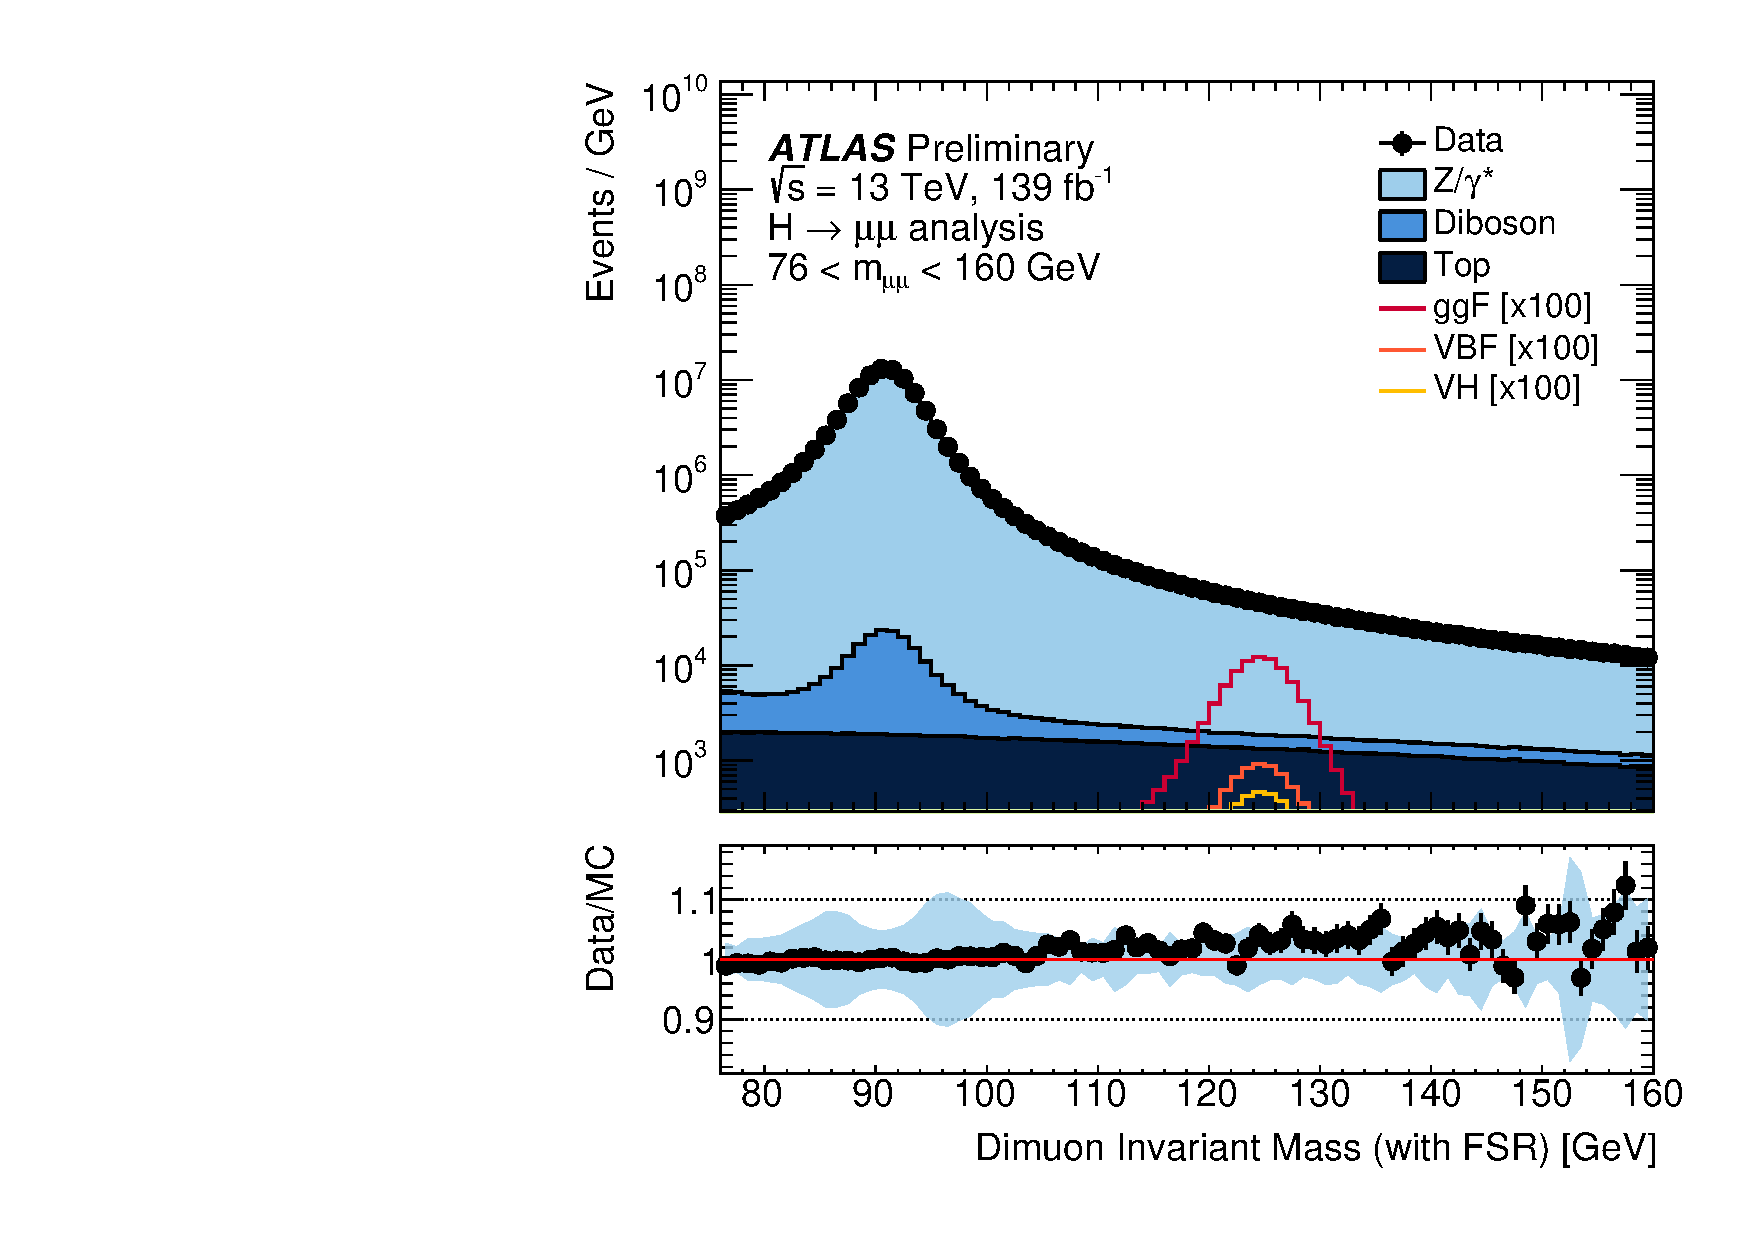
\includegraphics[width=0.9\textwidth]{figures/hmumu/sel-mmumu}
  \caption[Dimuon invariant mass spectrum of selected events.]{
  The invariant mass spectrum after the correction for
  final state radiation, for data corresponding to 139 $\ifb$.
  MC simulation is normalised to the data for easier comparison.
  Data is shown as black markers, the MC simulation of backgrounds
   is dominated by the DY events (light blue),
  followed by diboson (blue) and top (dark blue) contributions.
  Signal events coming from the $\ggf$, VBF, and VH production
  modes are shown as solid red, orange, and yellow lines,
  respectively, with the yields normalised to one hundred times the
  SM prediction for visibility. There are too few $\tth$ events to appear
  on the figure. The bottom panel shows the ratio between the data
  and MC simulation of background events, while the blue band
  represents the experimental systematic uncertainty. Statistical
  uncertainty on both data and MC simulation is combined in the
  error bars on data. From Ref. \cite{ATLAS-CONF-2019-028}}
  \label{fig:hmumu:sel-mmumu}
\end{figure}

\section{Event categorisation}

The goal of event categorisation is to improve the sensitivity of the
analysis by splitting events in categories with different signal
purities. In previous iterations of the analysis physics-based
arguments were used to construct categories targeting the VBF 
production mode and signal enriched regions using requirements on
event kinematics. However, with increased statistics of the
available dataset it became increasingly advantageous to exploit
modern machine learning models and infer the classification scheme
from the available data. With this approach care needs to be taken
to prevent bias and sub-optimal performance due to overfitting.

The categorisation scheme begins by splitting events in categories
based on jet multiplicity: 0-jet, 1-jet, and 2-jet channel, where
the 2-jet channel includes events with more than two jets.
%\footnote{ A categorisation approach without this initial split was tested and
%results in a small ($\sim 1\%$) improvement, but the split was kept
%to minimise systematics from the modelling of jet multiplicity.}
Kinematic differences between signal and background events are
exploited by training boosted decision tree (BDT) classifiers in
each of the jet channels using the XGBoost \cite{Chen:2016:XST:2939672.2939785}
package.

In each of the categories a ``Higgs classifier" is trained to
distinguish between MC simulation of $\ggf$ and VBF events, and the
data events from the sideband region. In the 2-jet
category an additional ``VBF classifier" is trained to distinguish
between the MC simulation of VBF signal events, and the data sidebands.
In both trainings the signal event weights are scaled so that their sum
matches the number of data events. 

The variables used in the training in each of the jet channels are
summarised in Table \ref{tab:hmumu:variables}. 0-jet channel uses
only three variables, related to the kinematics of the dimuon system:
$\pt$ and rapidity in addition to $|\cos{\theta*}|$, a variable
sensitive to the spin of the mediator \cite{PhysRevD.16.2219,
Sirunyan:2018swq}. In 1-jet channel the set of variables is 
extended by adding the kinematics of the leading jet. In the 2-jet
channel the kinematics of the subleading jet are added, along with
$\met$ and a couple of variables related to the dijet system.
\begin{table}[h]
\centering
\caption{Summary of the training variables.}
\label{tab:hmumu:variables}
\begin{tabular}{c c c}
\toprule
\midrule
\multirow{3}{*}{0-jet} & $\pt^{\mu\mu}$      & $\pt$ of the dimuon system \\
                       & $Y^{\mu\mu}$        & Rapidity of the dimuon system\\
                       & $|\cos{\theta*}|$   & Spin-related variable \\
\midrule
\multirow{4}{*}{1-jet} & 0-jet variables            &  \\
                       & $\pt^{j_1}$                & $\pt$ of the lead jet \\
                       & $\eta^{j_1}$               & $\eta$ of the lead jet \\
                       & $\Delta \phi_{j_1,\mu\mu}$ & $\Delta \phi$ between the lead jet and dimuon system \\
\midrule
\multirow{9}{*}{2-jet} & 1-jet variables            &  \\
                       & $\pt^{j_2}$                & $\pt$ of the sublead jet \\
                       & $\eta^{j_2}$               & $\eta$ of the sublead jet \\
                       & $\Delta \phi_{j_2,\mu\mu}$ & $\Delta \phi$ between the sublead jet and dimuon system \\
                       & $\pt^{jj}$                 & $\pt$ of the dijet system \\
                       & $Y^{j_2}$                  & Rapidity of the dijet system \\
                       & $\Delta \phi_{jj,\mu\mu}$  & $\Delta \phi$ between the dijet system and dimuon system \\
                       & $m_{jj}$                   & Invariant mass of the dijet system \\
                       & $\met$                     & Missing transverse energy \\
\midrule
\bottomrule
\end{tabular}
\end{table}

The variables were chosen to maximise the sensitivity while
minimising systematic uncertainties. An additional concern was
whether the variables would allow the classifier to learn the
invariant mass and result in a shaped mass spectrum after selection.
For this reason the complete kinematics of the individual muons
are not included.

All the variables used in the 2-jet channel are shown in Figures
\ref{fig:hmumu:variables01} and \ref{fig:hmumu:variables2} for
events with two or more jets. It can be seen that the $\pt$ of
the dimuon system, mass of the dijet system and azimuthal
differences between the dimuon system and jets can provide
separation between the signal and the background.

\begin{figure}[h!]
  \centering
  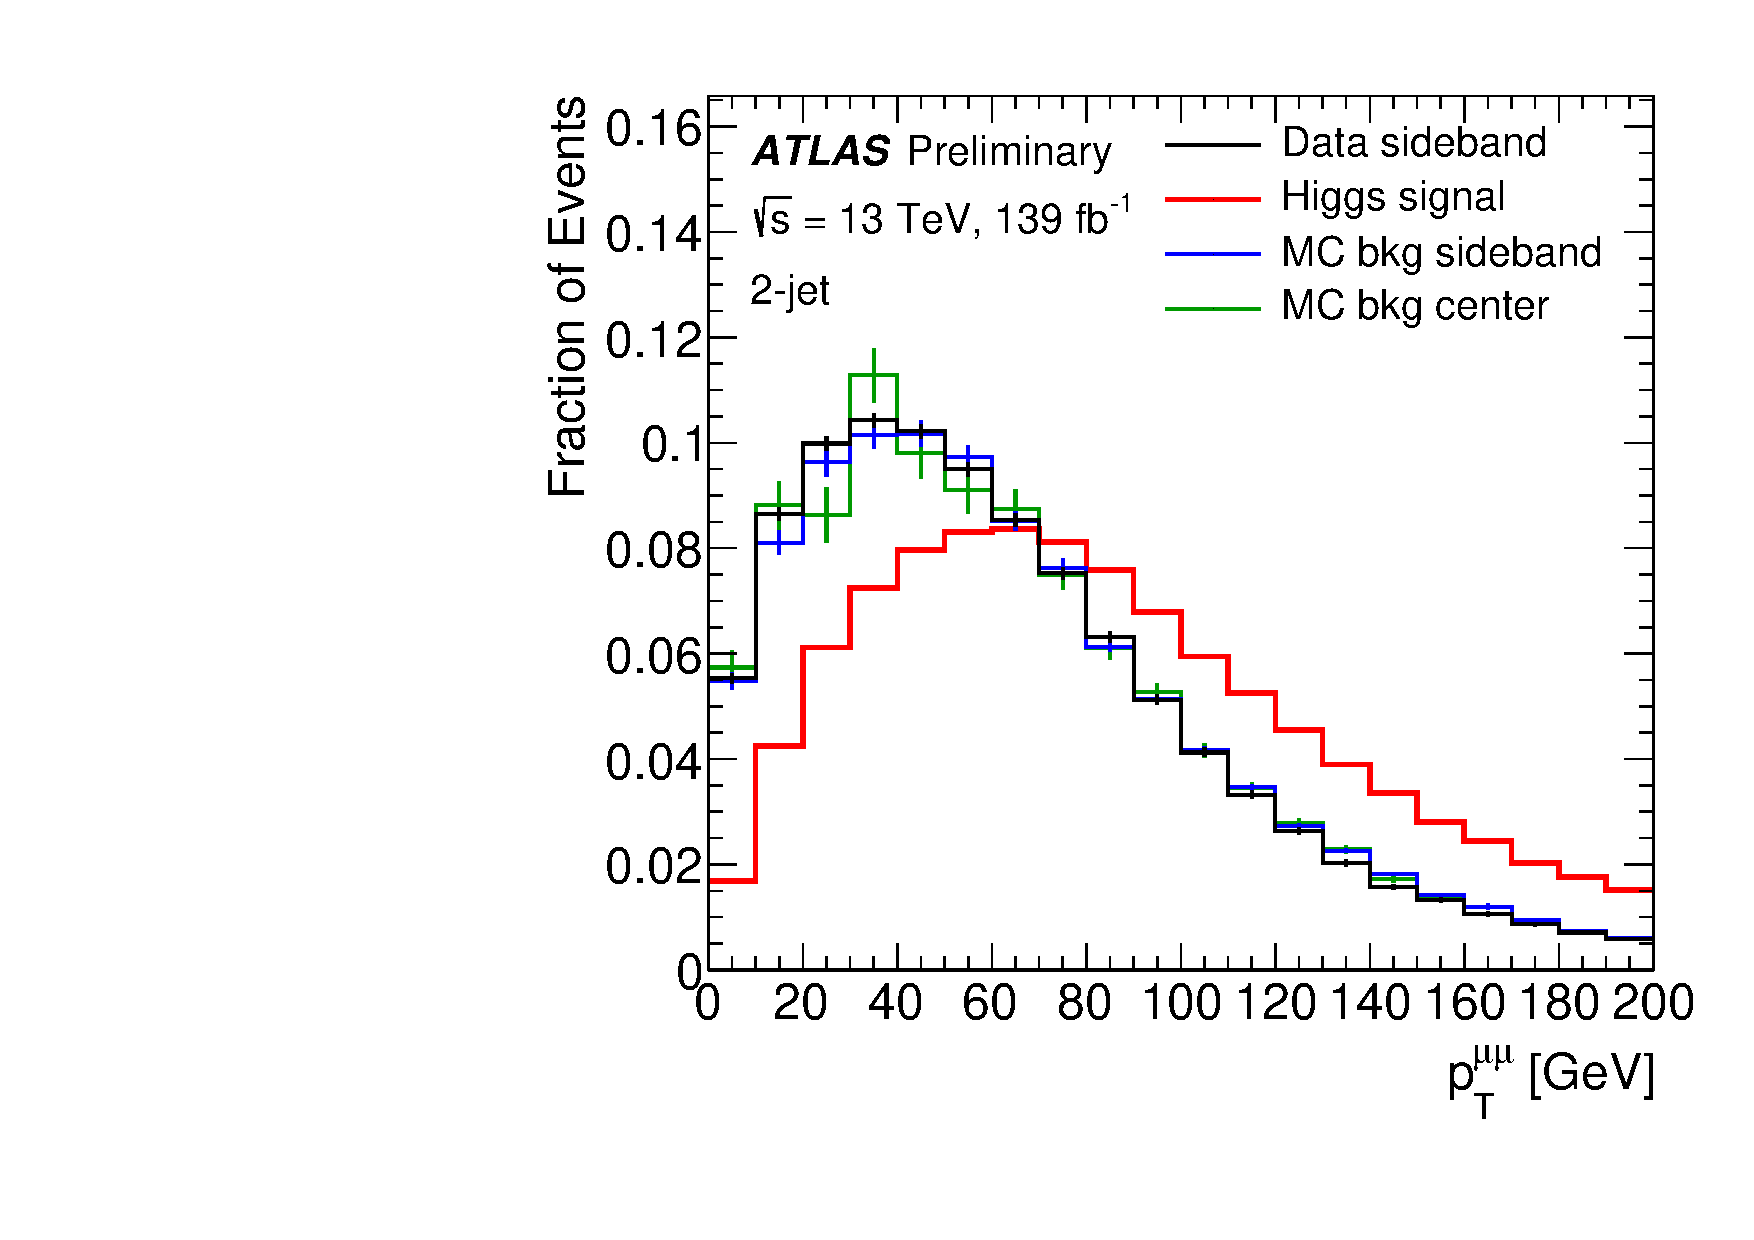
\includegraphics[width=0.3\textwidth]{figures/hmumu/vars/Z_PT_FSR}
  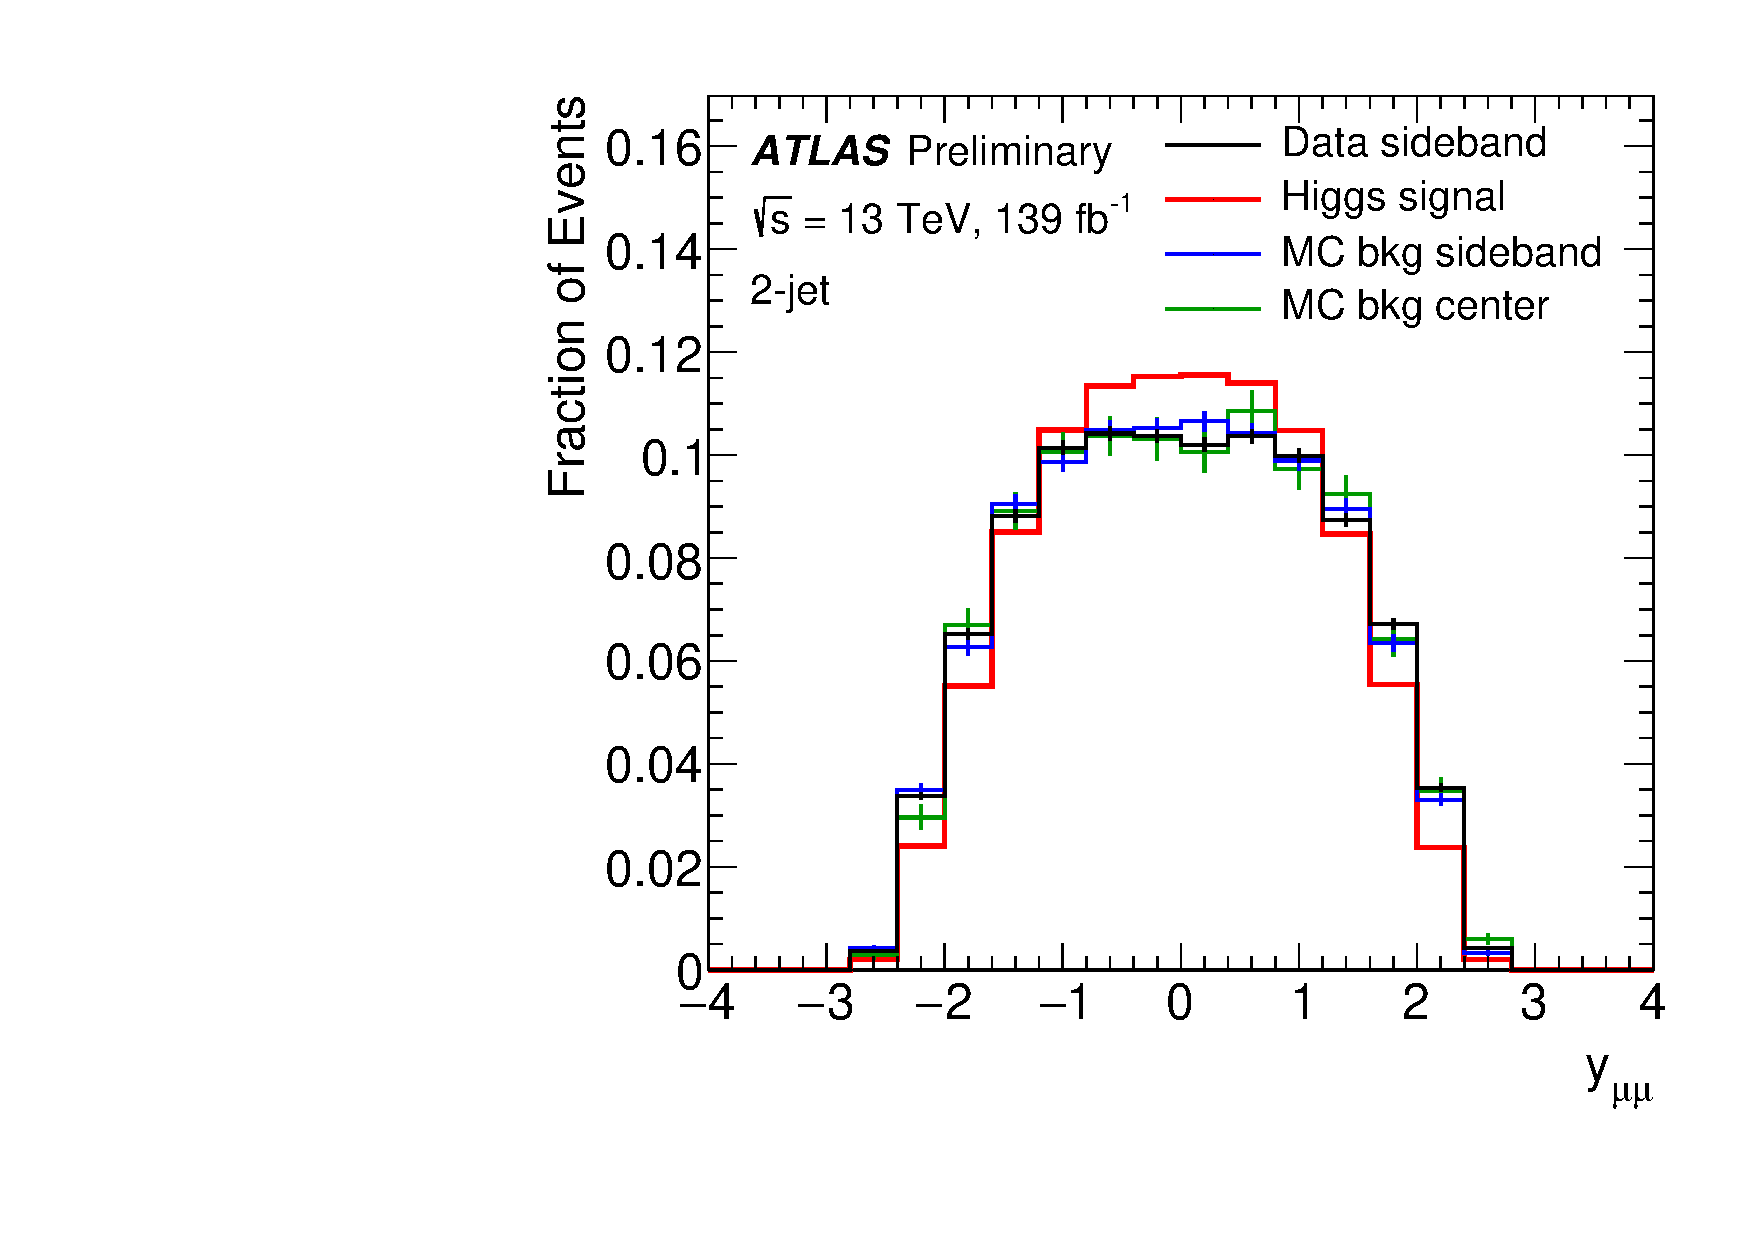
\includegraphics[width=0.3\textwidth]{figures/hmumu/vars/Z_Y_FSR}
  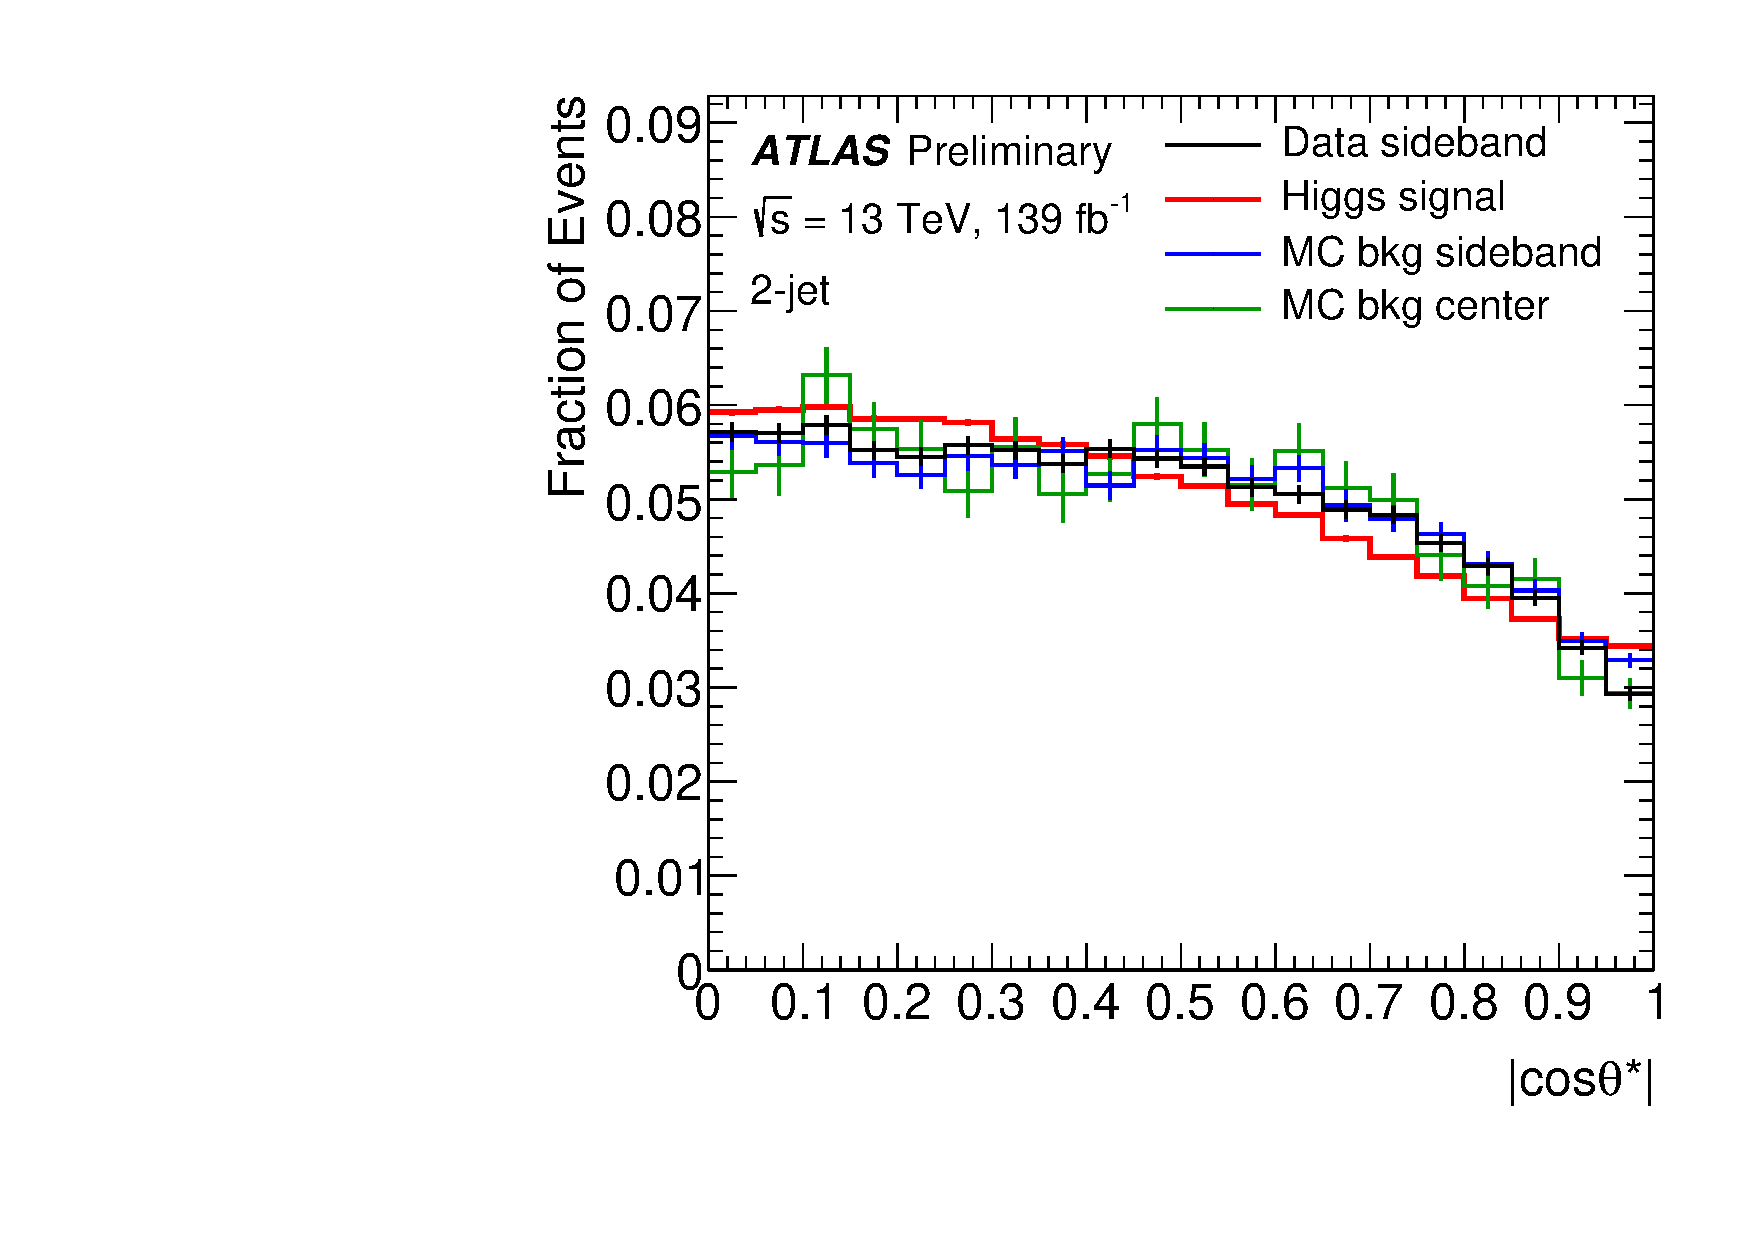
\includegraphics[width=0.3\textwidth]{figures/hmumu/vars/CosThetaStar} \\ 
  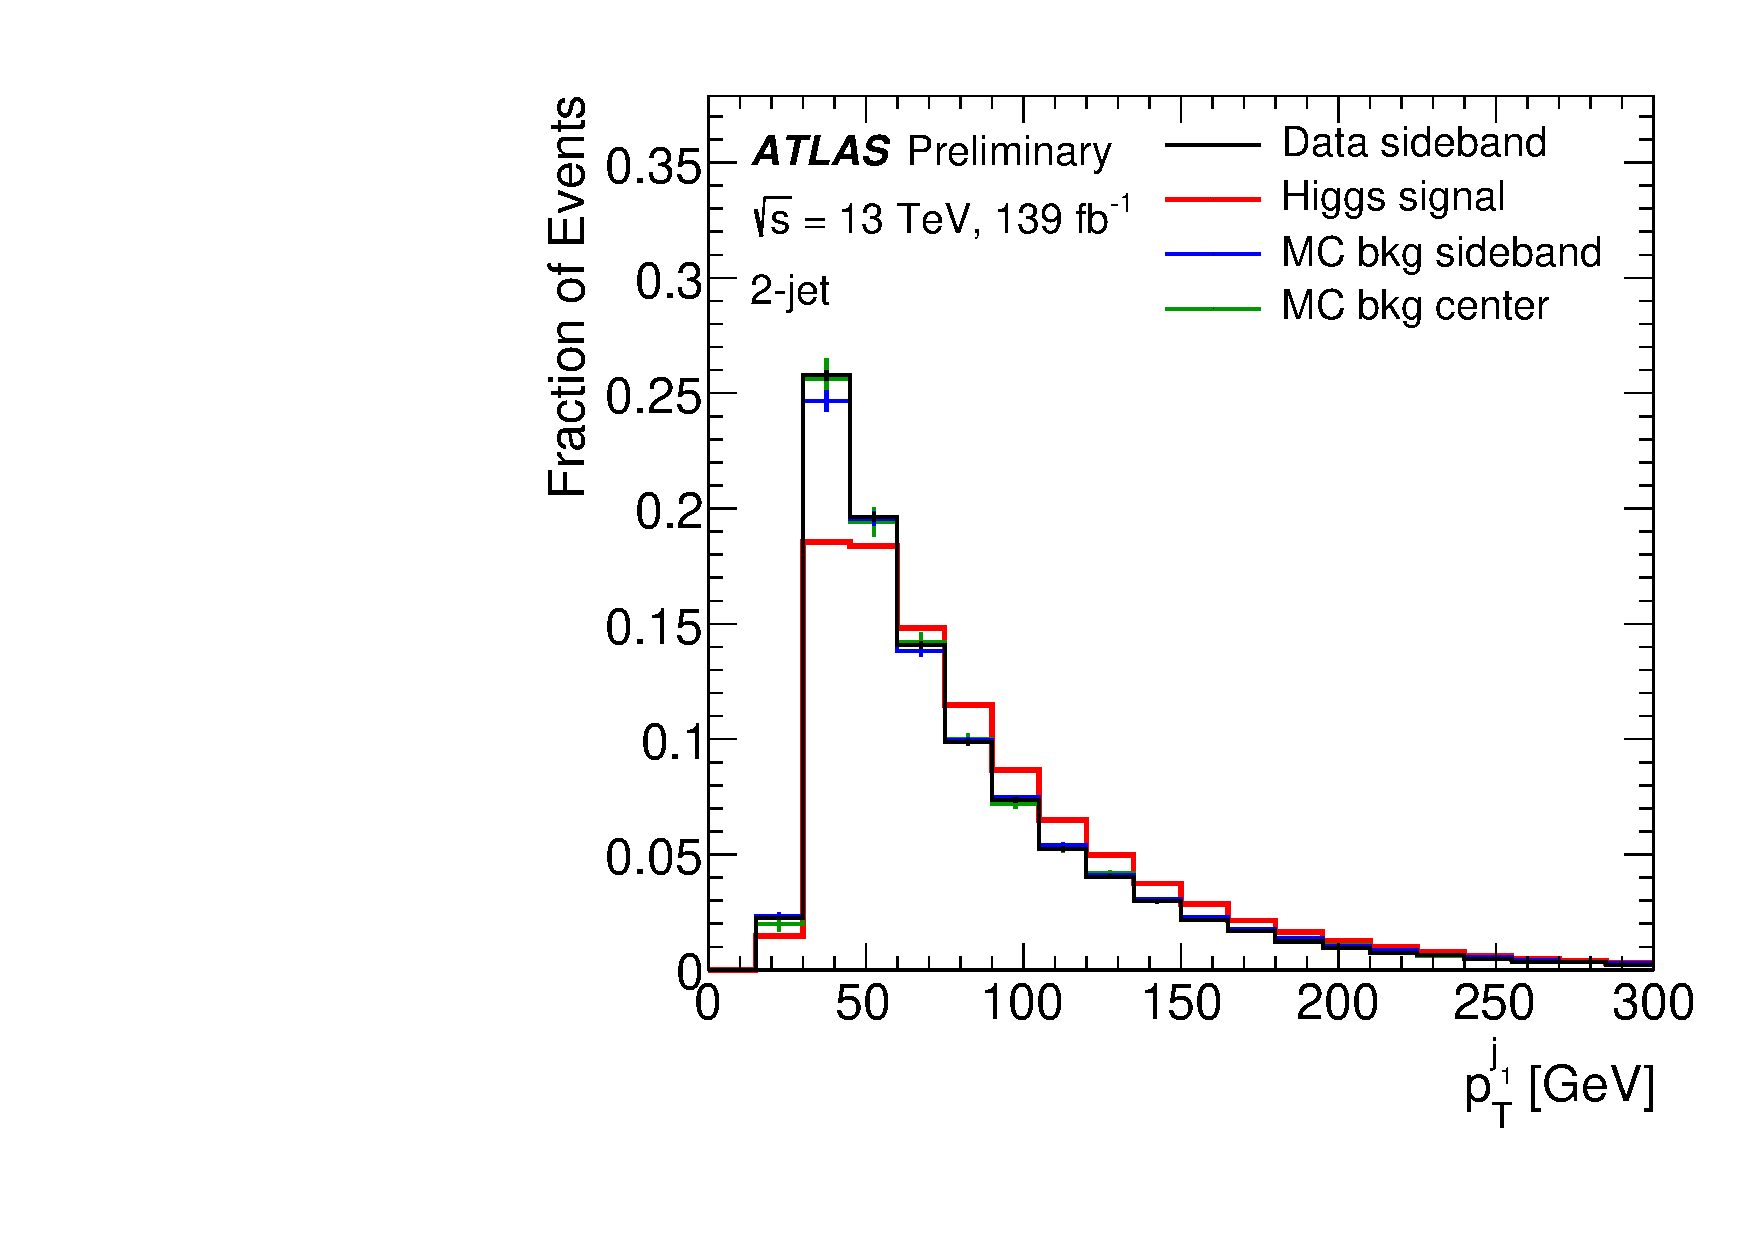
\includegraphics[width=0.3\textwidth]{figures/hmumu/vars/Jets_PT_Lead}
  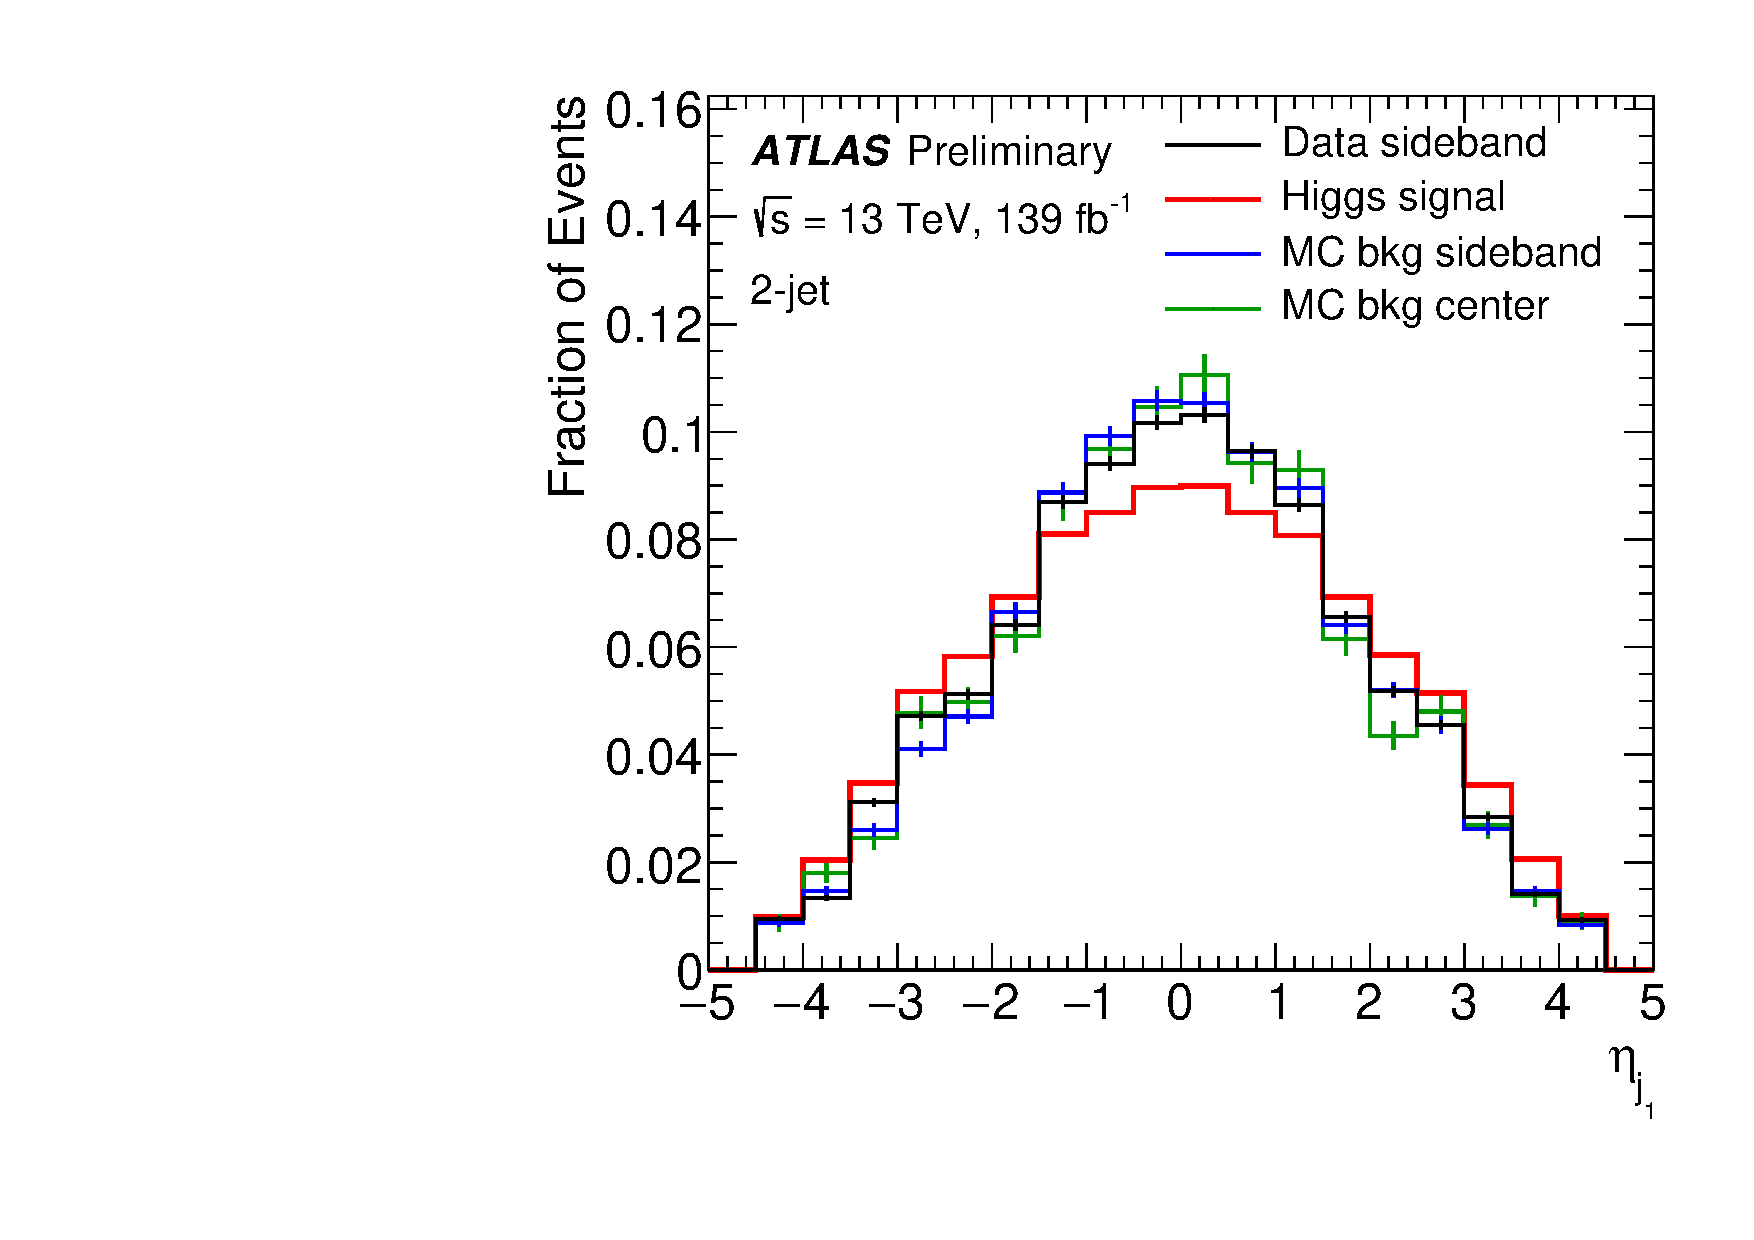
\includegraphics[width=0.3\textwidth]{figures/hmumu/vars/Jets_Eta_Lead}
  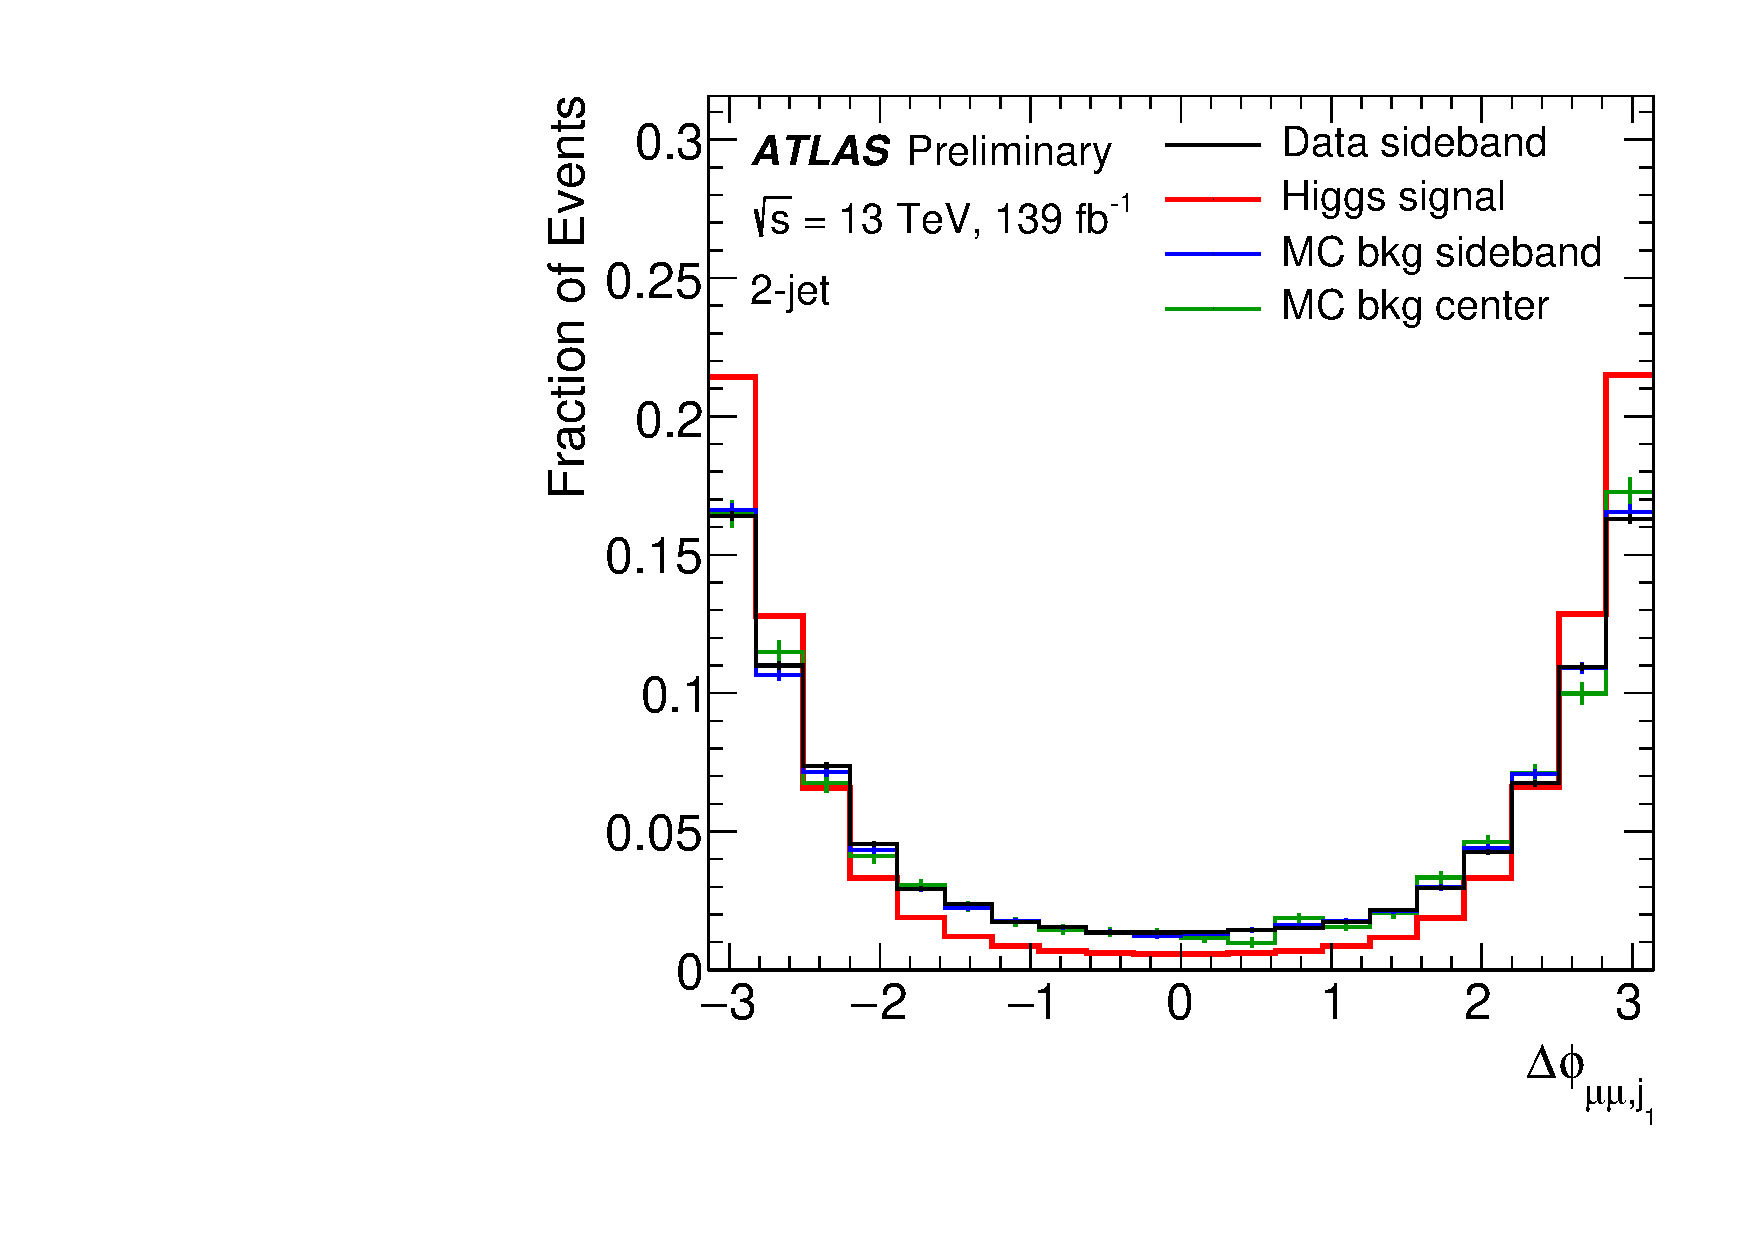
\includegraphics[width=0.3\textwidth]{figures/hmumu/vars/DeltaPhi_mumuj1} \\ 
  \caption[Classifier input variables]{
  Distributions of classifier
  input variables for events with two or more jets. Top row shows dimuon
  system variables, bottom row shows leading jet variables. $\hmumu$ signal events
  are shown in red, data from the sidebands are shown in black, and MC
  simulation of background events is shown blue (sideband region) and
  green (central region). MC simulation includes DY, diboson, and top events.
  Error bars are statistical. From Ref. \cite{ATLAS-CONF-2019-028}.
  }
  \label{fig:hmumu:variables01}
\end{figure}

\begin{figure}[h!]
  \centering
  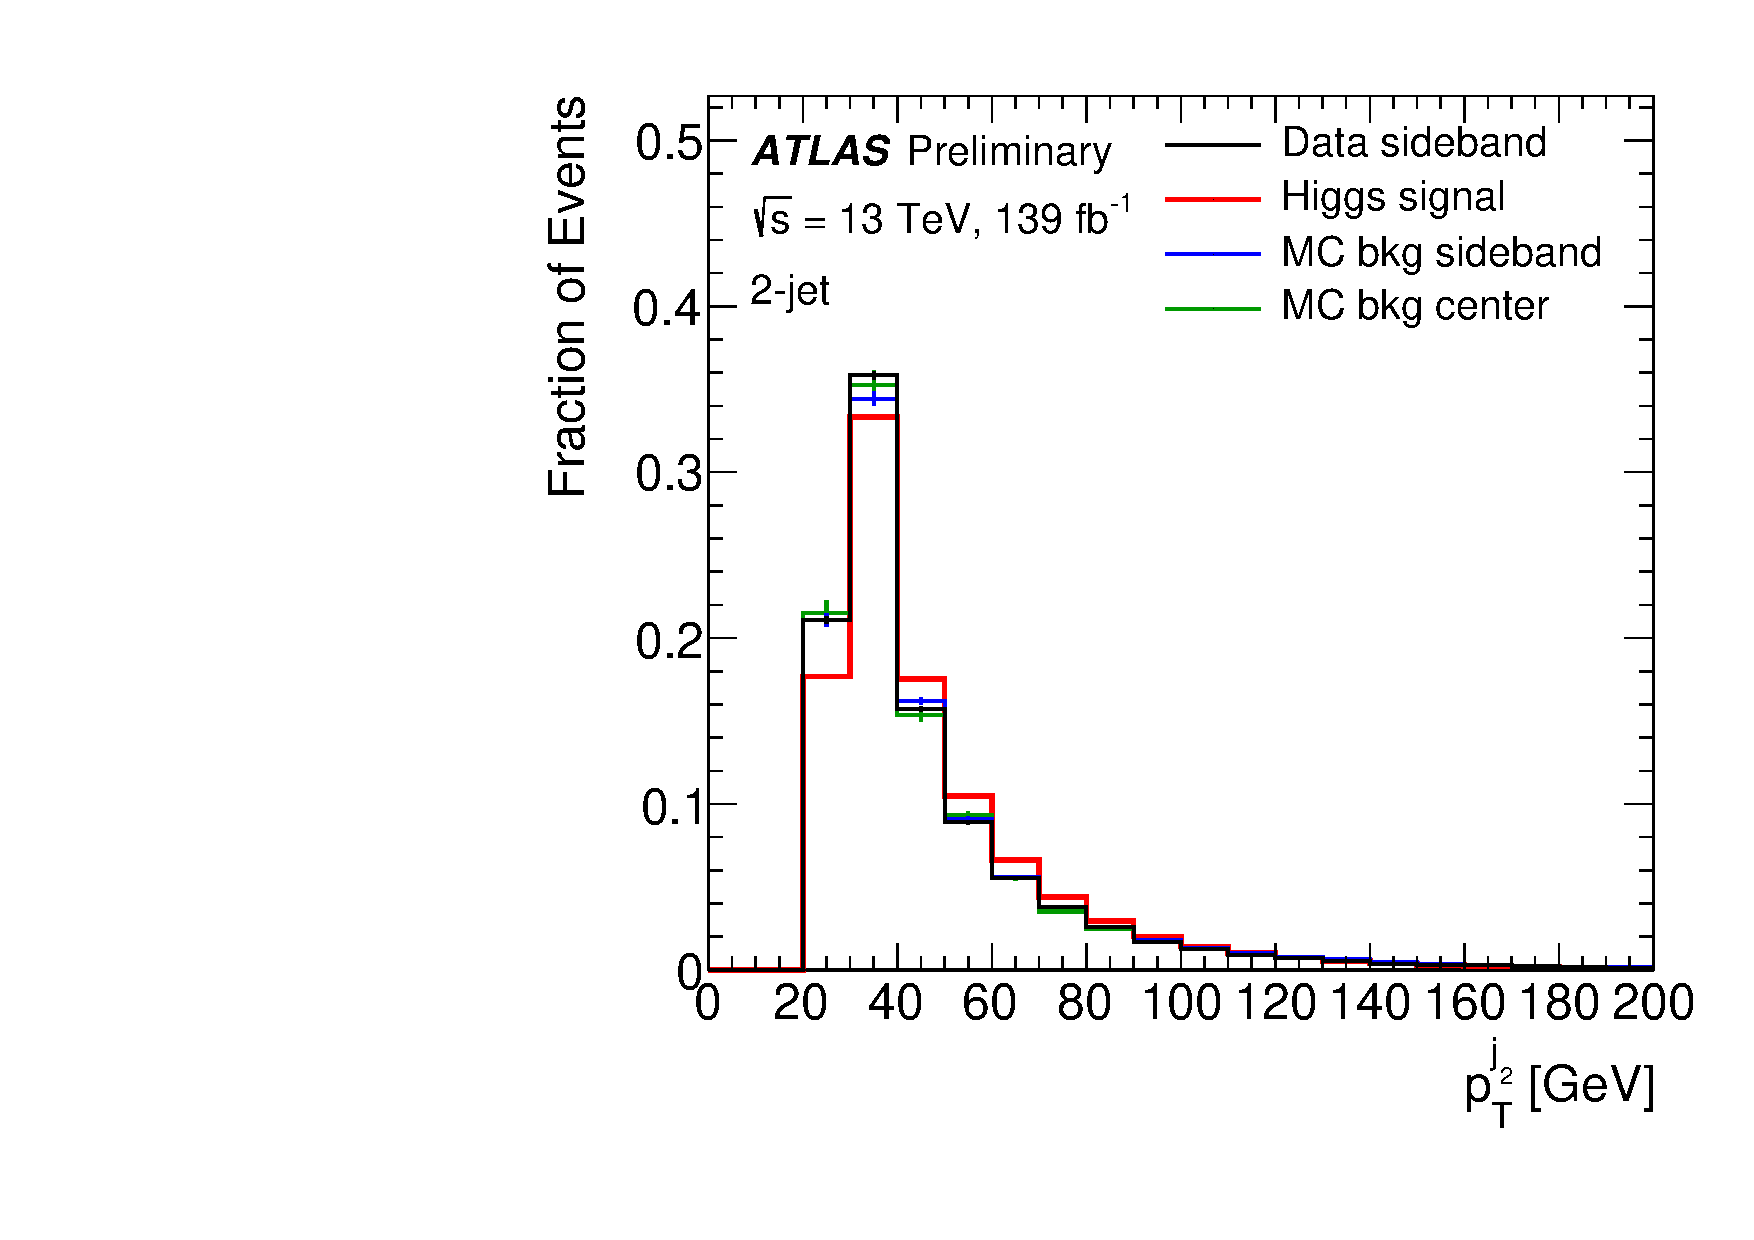
\includegraphics[width=0.3\textwidth]{figures/hmumu/vars/Jets_PT_Sub}
  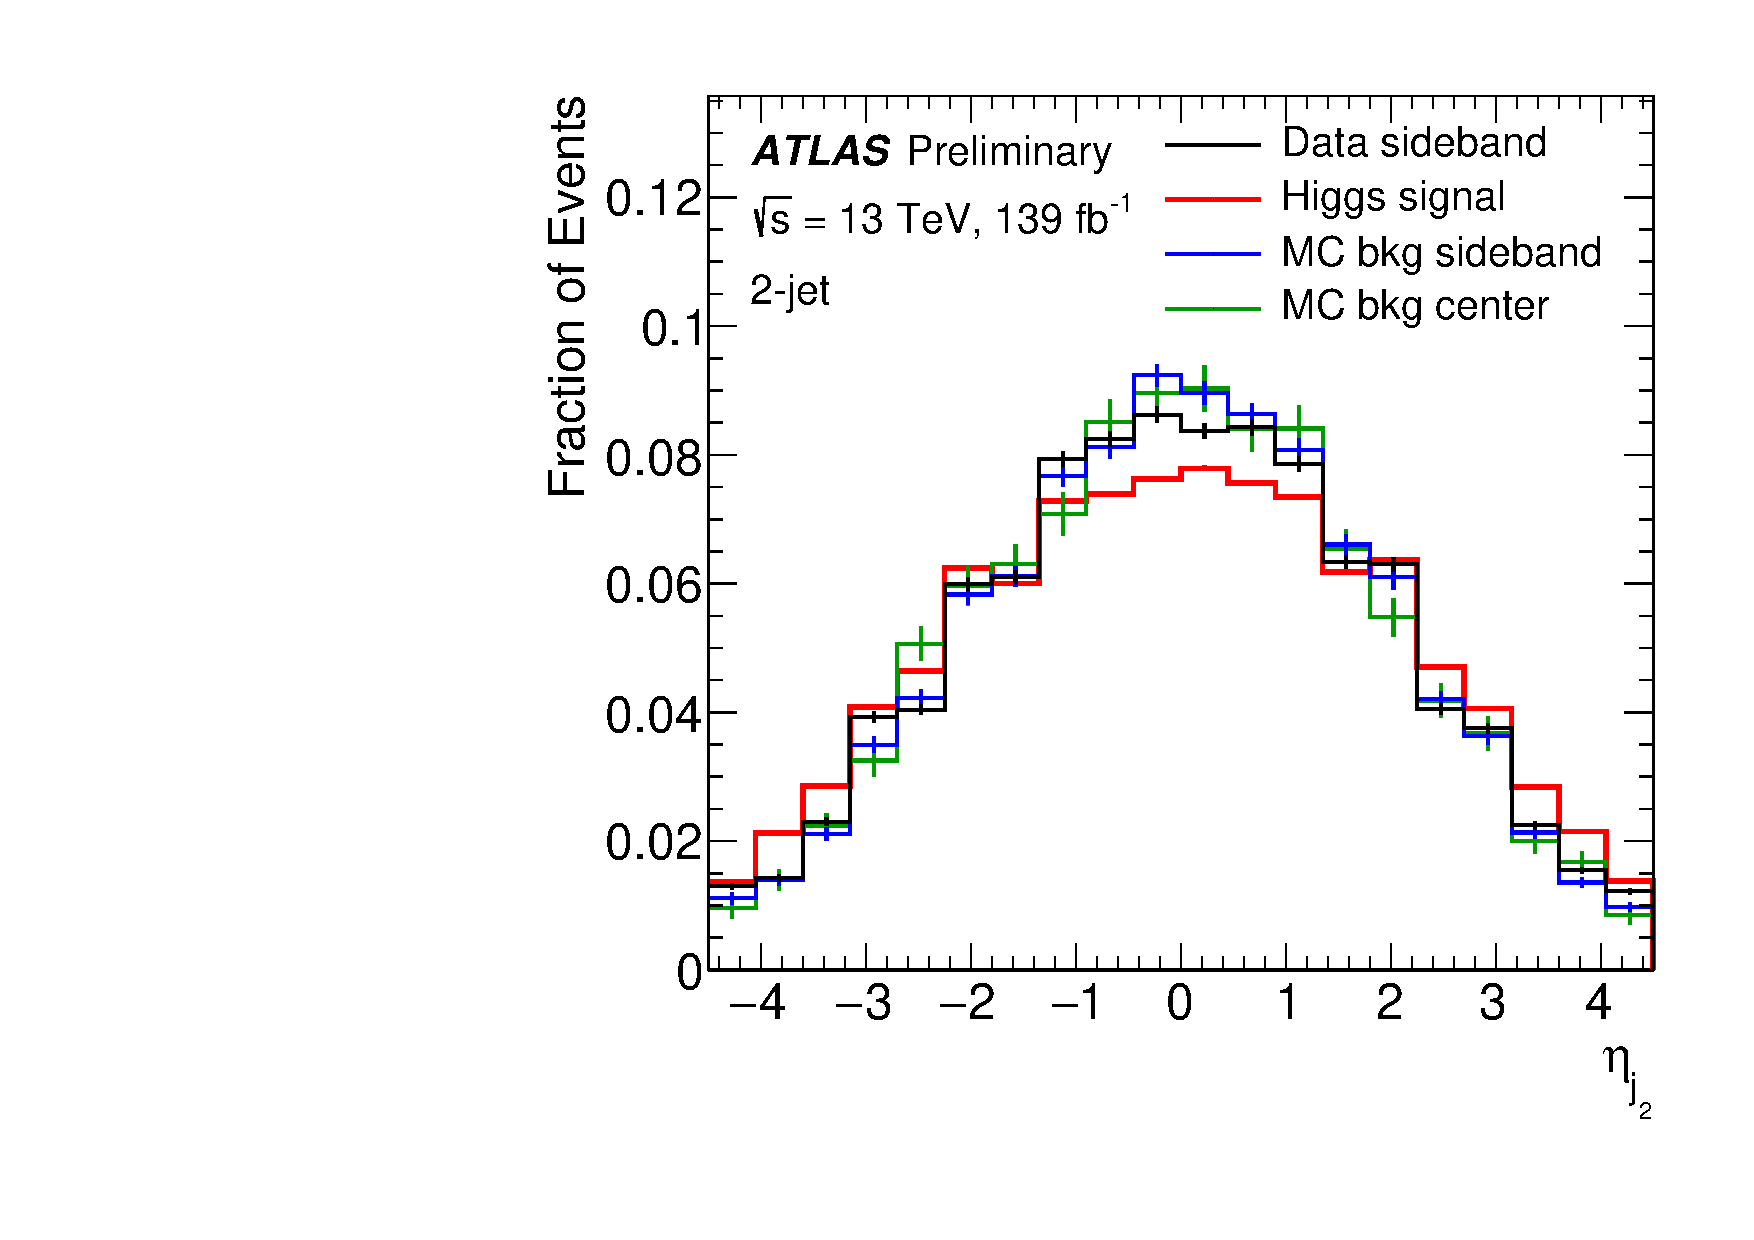
\includegraphics[width=0.3\textwidth]{figures/hmumu/vars/Jets_Eta_Sub}
  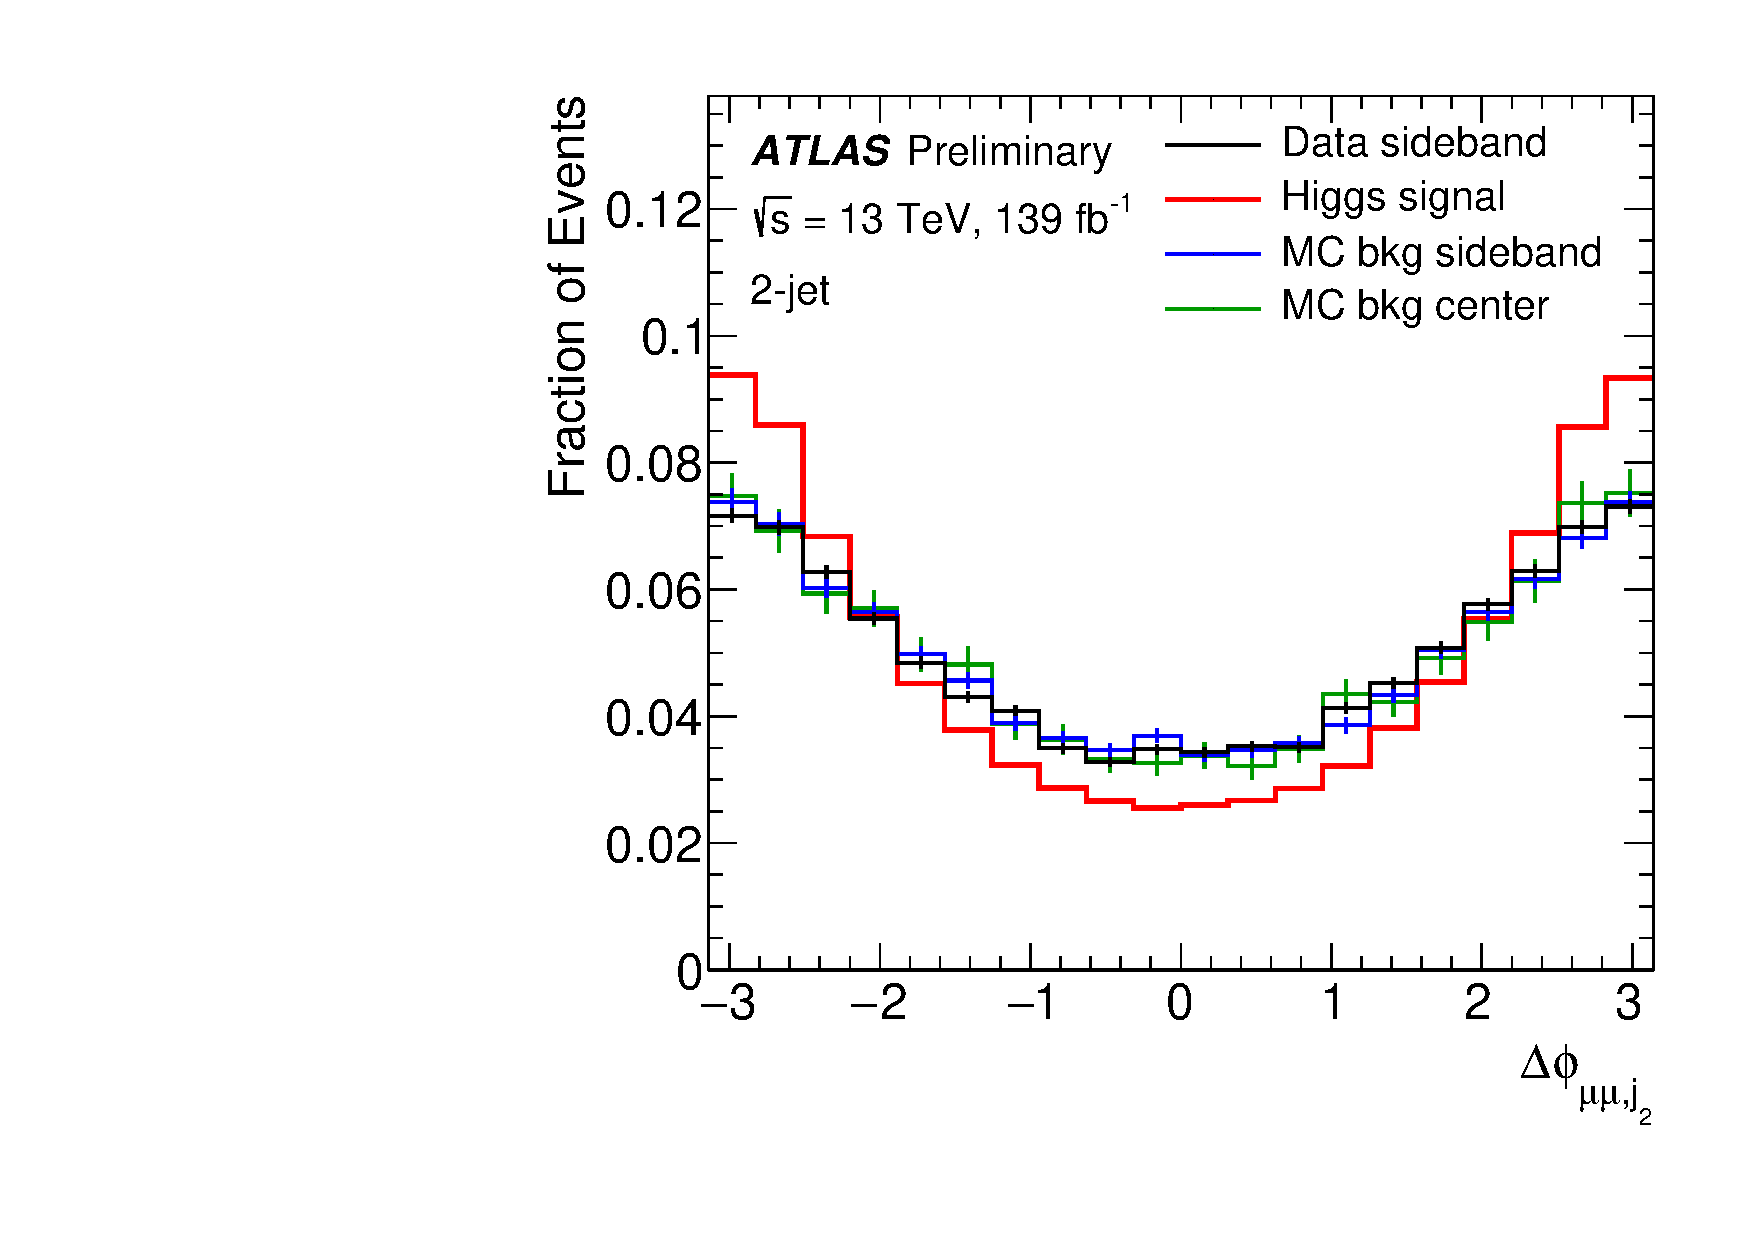
\includegraphics[width=0.3\textwidth]{figures/hmumu/vars/DeltaPhi_mumuj2} \\
  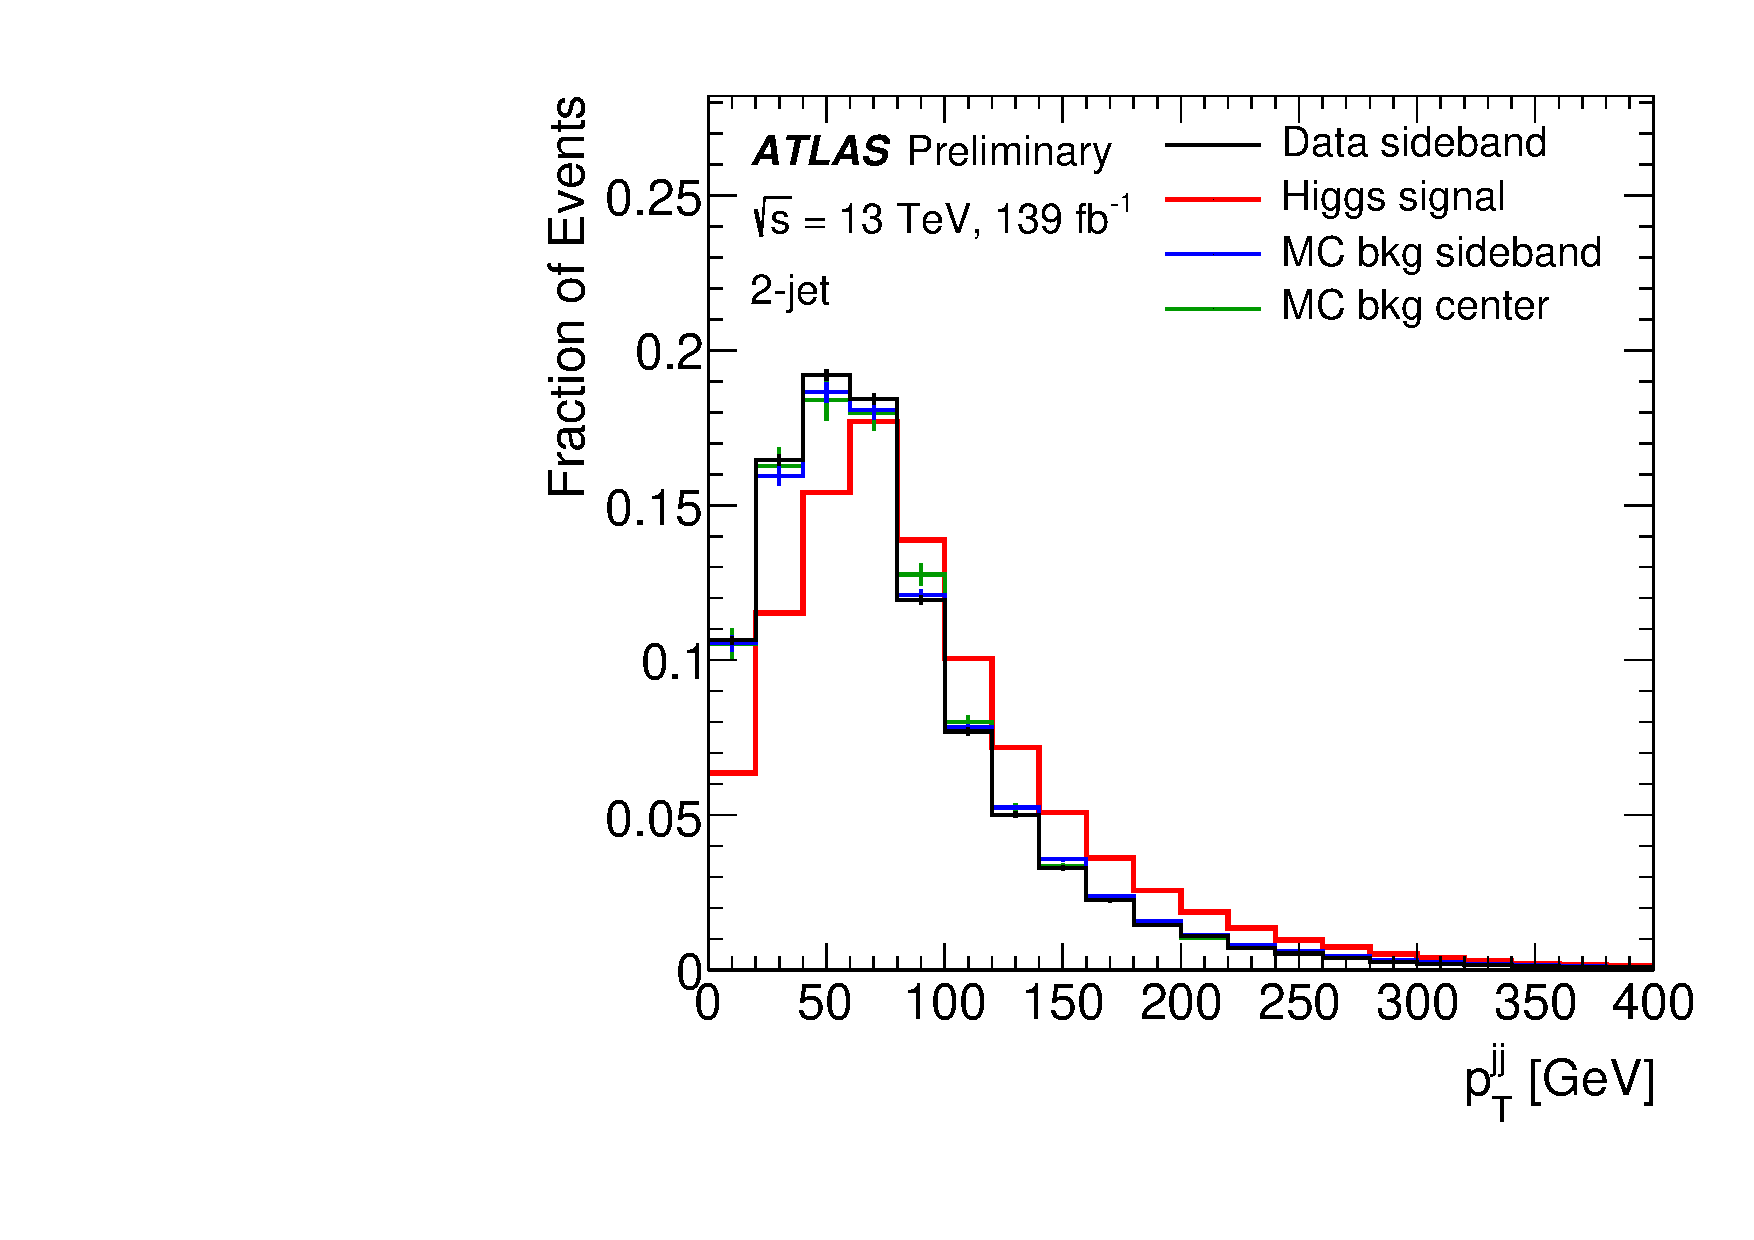
\includegraphics[width=0.3\textwidth]{figures/hmumu/vars/Jets_PT_jj}
  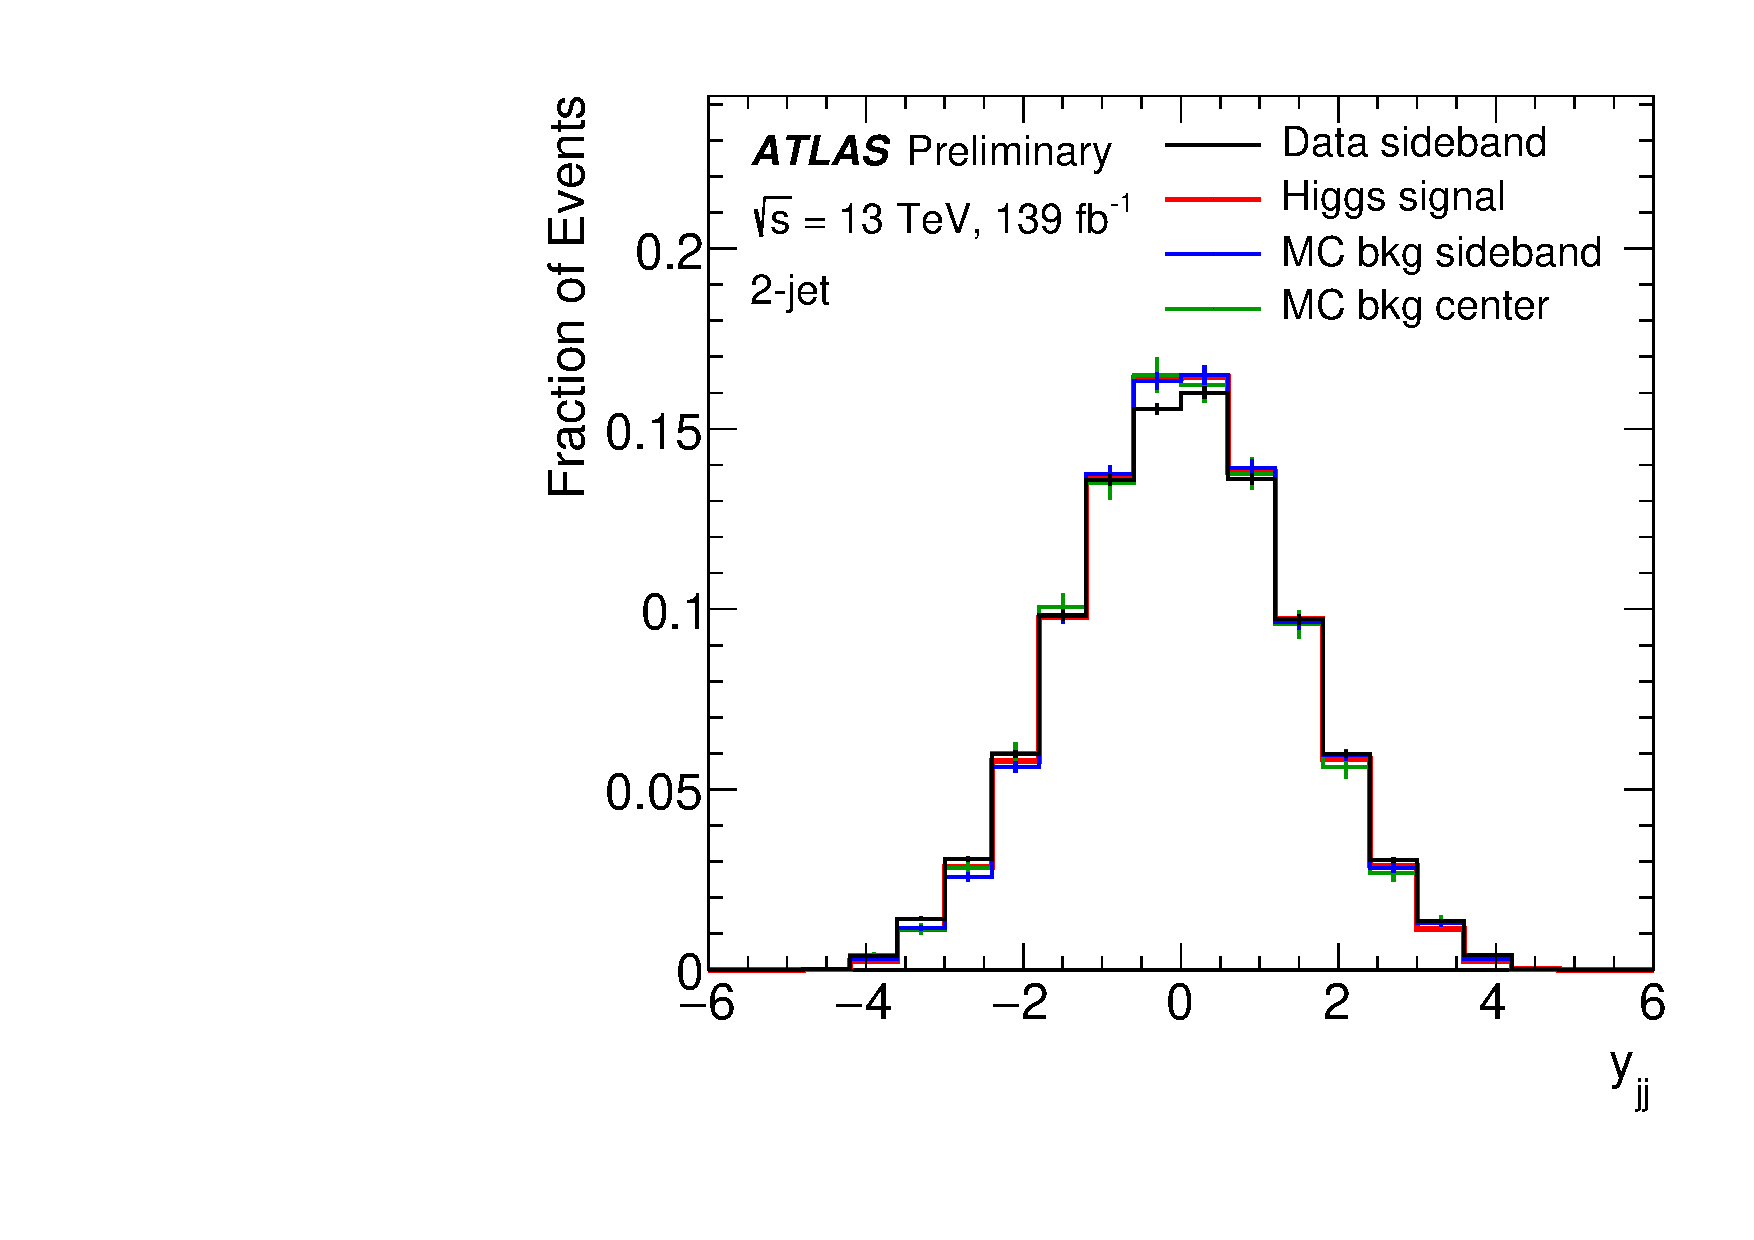
\includegraphics[width=0.3\textwidth]{figures/hmumu/vars/Jets_Y_jj}
  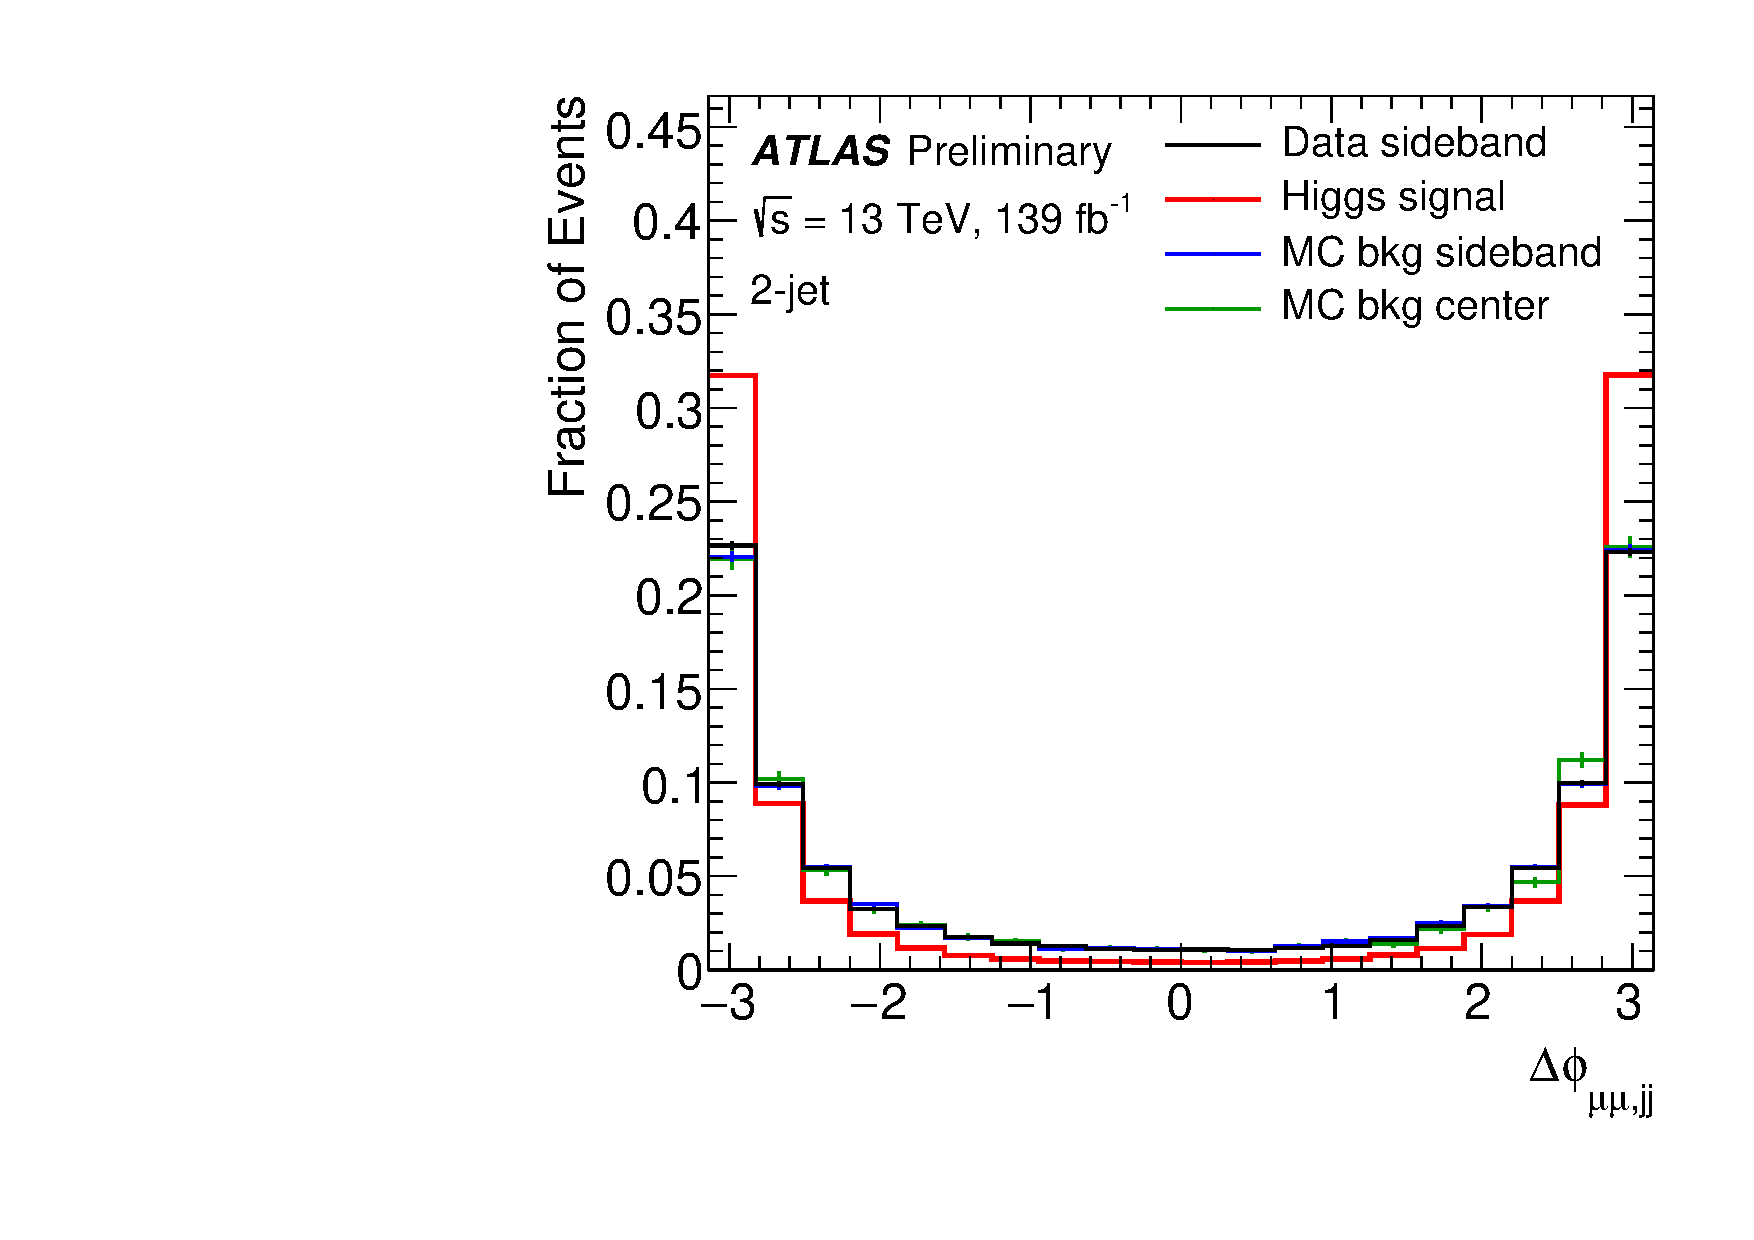
\includegraphics[width=0.3\textwidth]{figures/hmumu/vars/DeltaPhi_mumujj} \\
  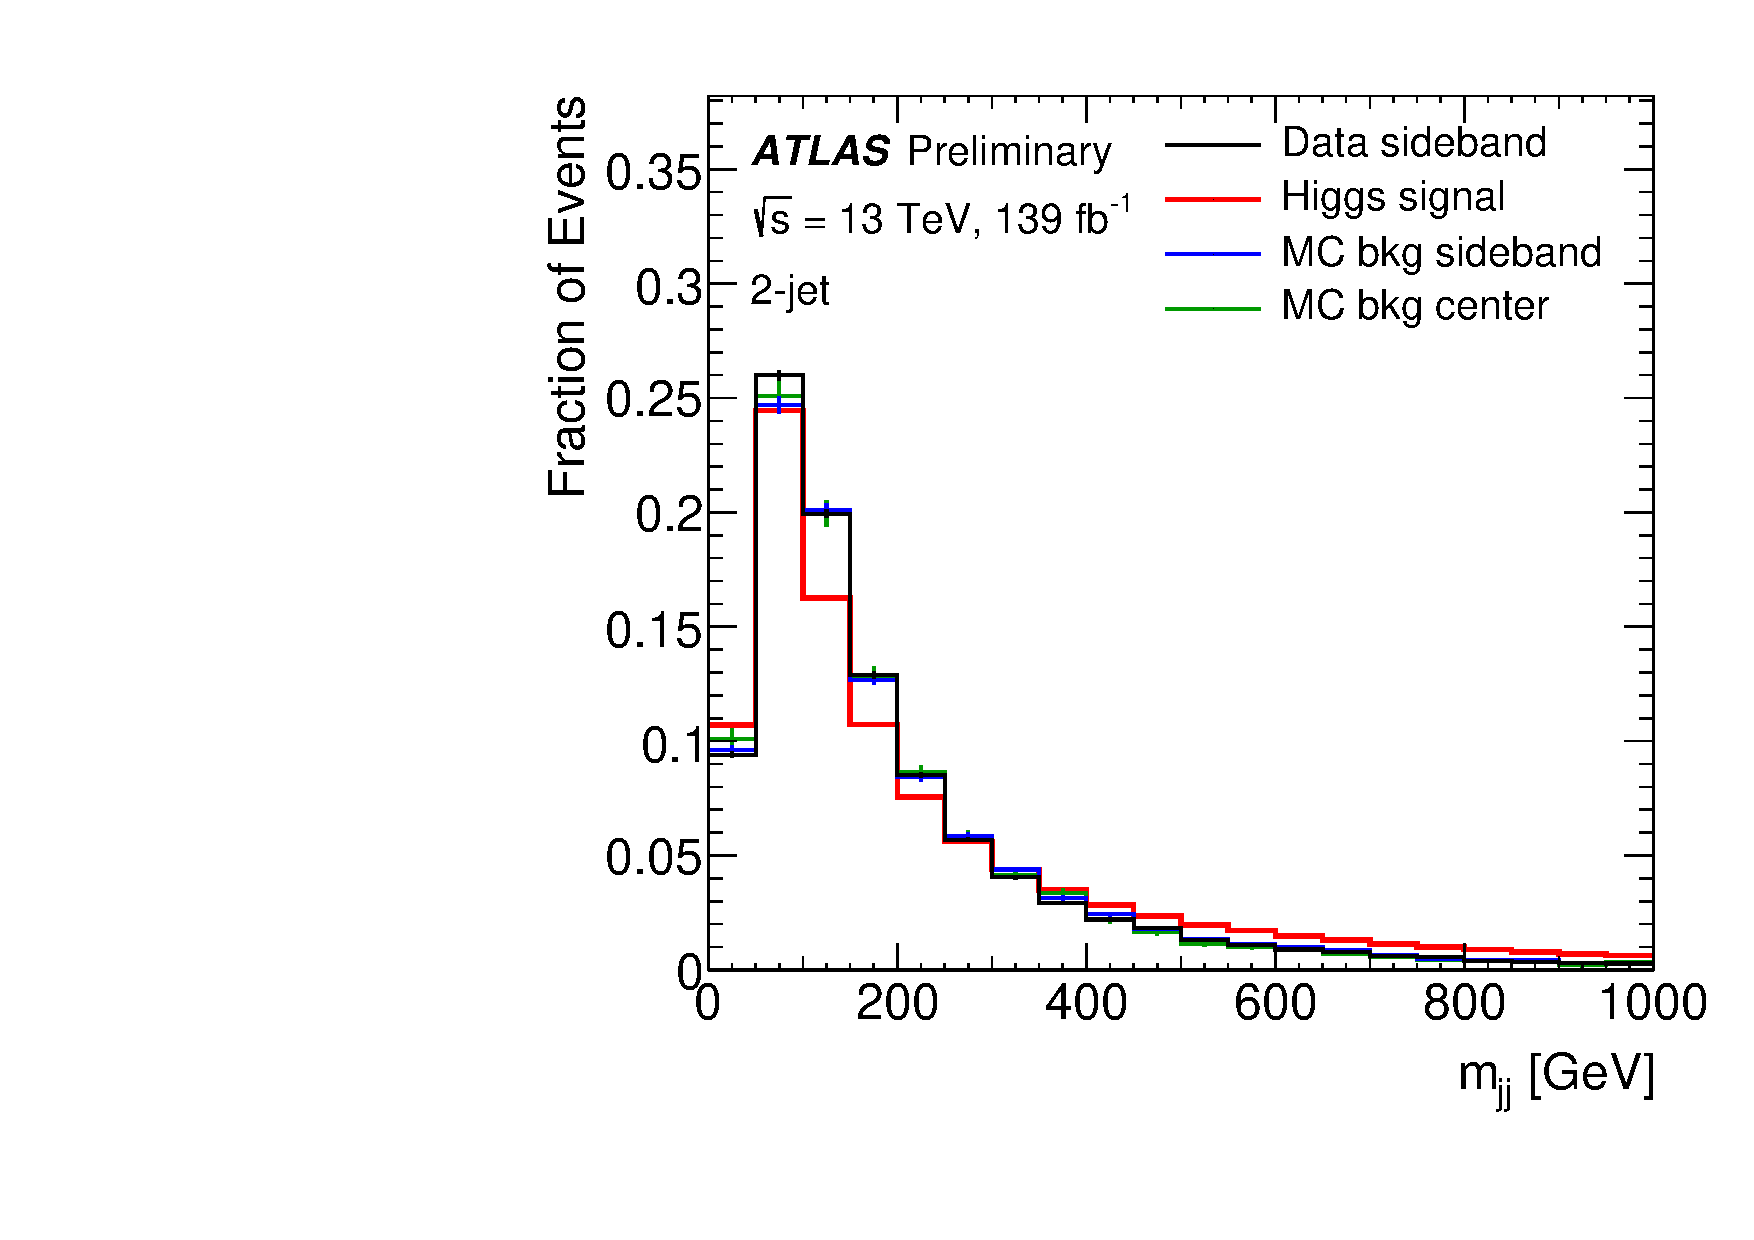
\includegraphics[width=0.3\textwidth]{figures/hmumu/vars/Jets_Minv_jj}
  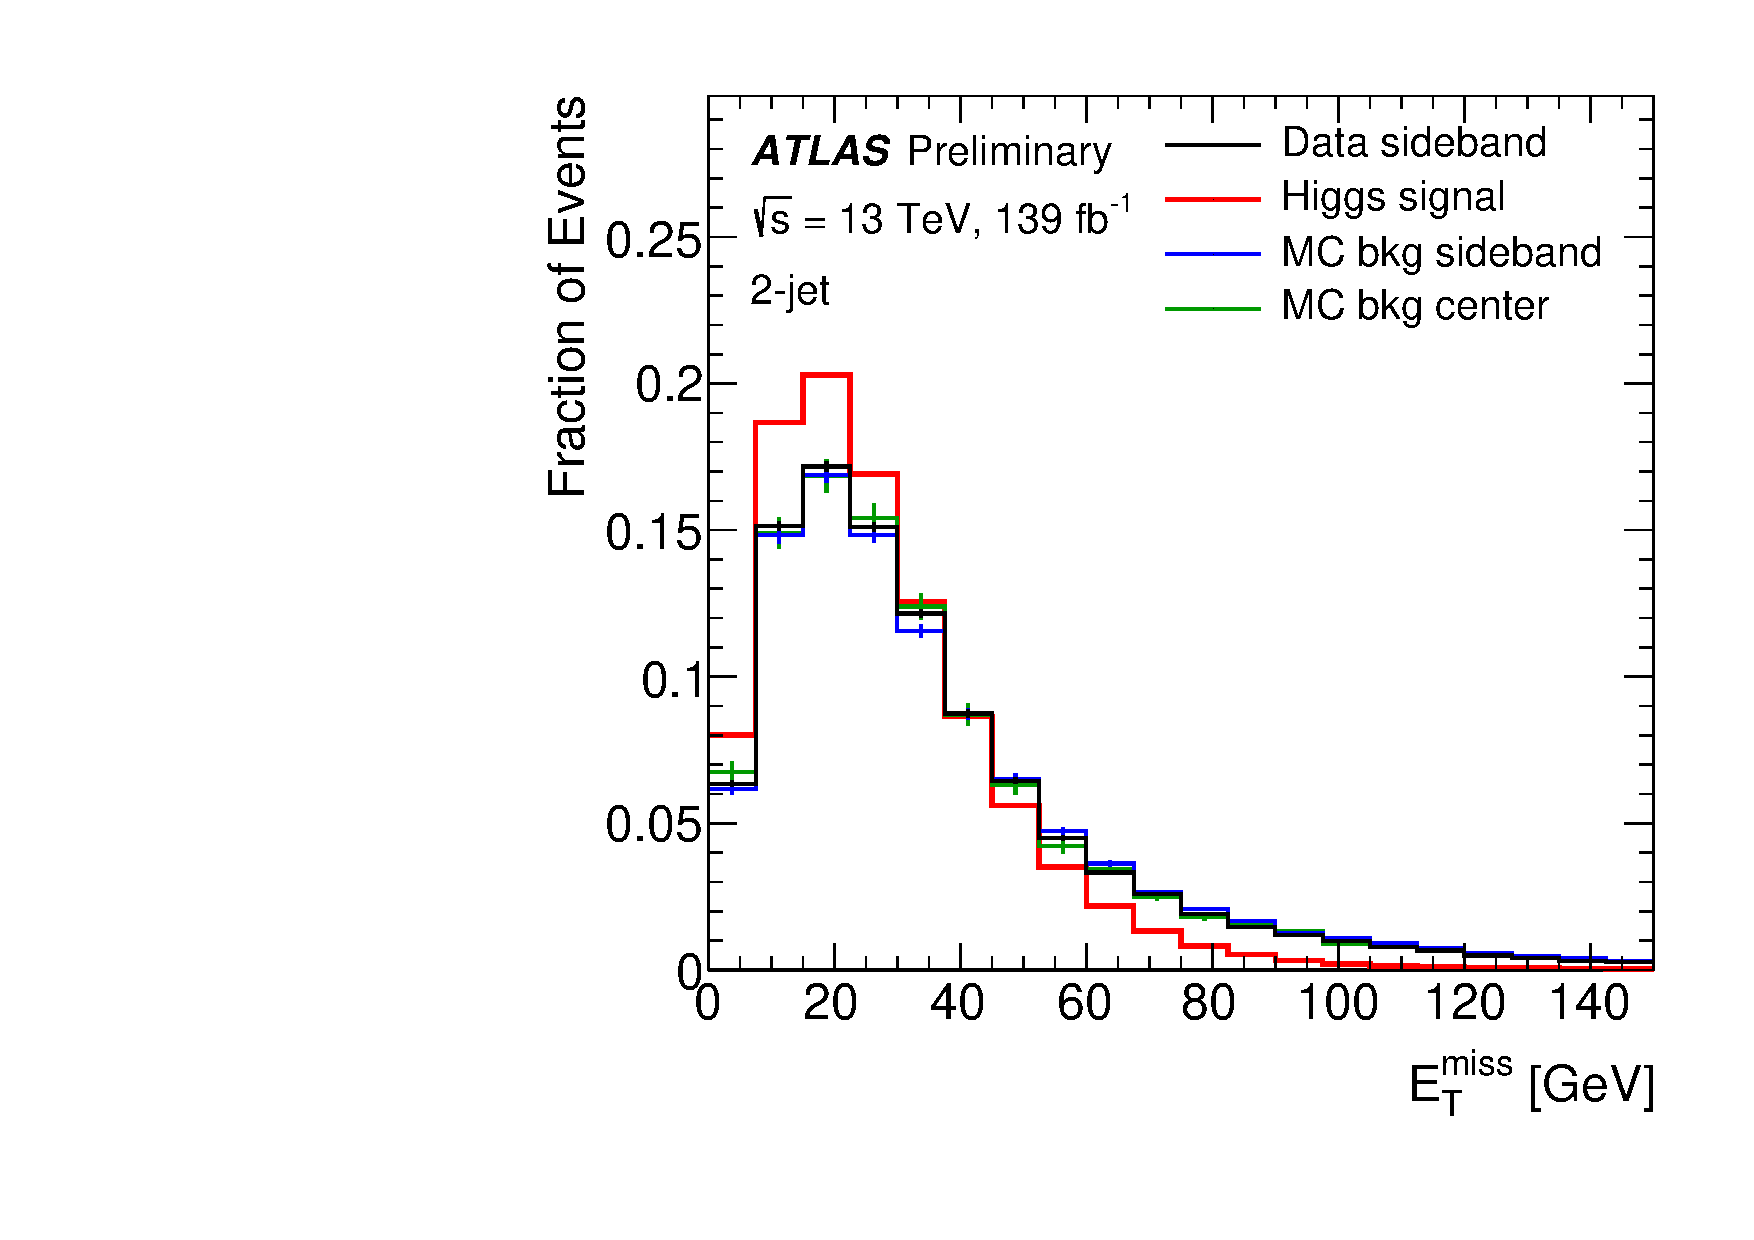
\includegraphics[width=0.3\textwidth]{figures/hmumu/vars/metFinalTrk}
  \caption[Classifier input variables]{
  Distributions of classifier
  input variables for events with two or more jets. Top row shows subleading
  jet variables, middle row dijet system variables, bottom row shows the
  dijet invariant mass and $\met$. $\hmumu$ signal events
  are shown in red, data from the sidebands are shown in black, and MC
  simulation of background events is shown blue (sideband region) and
  green (central region). MC simulation includes DY, diboson, and top events.
  Error bars are statistical. From Ref. \cite{ATLAS-CONF-2019-028}.
  }
  \label{fig:hmumu:variables2}
\end{figure}

In each jet multiplicity channel a four-fold approach is used to
prevent bias from overfitting to the training and validation sets.
In each fold, events are split in a training set (50\% of events),
a validation set (25\% of events), and a test set (25\% of events).
Training set is used in the training of the models. The validation
set is used for early stopping of the training and to assess the
performance of models using the area under the ROC
\cite{journals/prl/Fawcett06} curve. This is used to guide the
Bayesian optimisation \cite{gp} to tune the hyperparameters of the
model in each fold. Finally, the model is evaluated on the test set,
which is used for the categorisation of events.

It should be noted that in the four-fold approach the model parameters
are selected separately in each fold. This results in four models,
each being applied to the test set not seen in training, early stopping,
or hyperparameter tuning, ensuring that there is no bias from overfitting
to either training or validation datasets.

In order to ensure that the score distributions are the same in each
fold, the scores are transformed to a uniform distribution in unweighted
combined signal events in all fold separately using the QuantileTransformer
algorithm from the \texttt{scikit-learn} \cite{scikit-learn} software package.

The transformed scores are named $O_\text{VBF}$ for the VBF classifier,
and $O_\ggf^(0-2)$ for the Higgs classifiers, where the superscript
stands for the jet multiplicity. The category boundaries are defined
as the cuts on these values, and are summarised in Table \ref{tab:hmumu:categories}.
\begin{table}[h]
\centering
\caption{Summary of the score boundaries defining the analysis categories.}
\label{tab:hmumu:categories}
\begin{tabular}{c c c c}
\toprule
\midrule
%       &    0-jet                       &      1-jet                     & 2-jet ($O_\text{VBF} < 0.60$) & VBF \\
%High   & $O^0_{\ggf} \geq 0.75$         & $O^1_{\ggf} \geq 0.78$         & $O^2_{\ggf} \geq 0.48$          & $O_\text{VBF} \geq 0.89$ \\
%Medium & $0.35 \leq O^0_{\ggf} < 0.75$  & $0.38 \leq O^1_{\ggf} < 0.78$  & $0.22 \leq O^2_{\ggf} < 0.48$   & $0.77 \leq O_\text{VBF} < 0.89$ \\
%Low    & $O^0_{\ggf} < 0.35$            & $O^1_{\ggf} < 0.38$            & $O^2_{\ggf} < 0.22$             & $O_\text{VBF} < 0.77$ \\
                              & Low                   &  Medium                           &    High                  \\ 
\midrule
0-jet                         & $O^0_{\ggf} < 0.35$   &  $0.35 \leq O^0_{\ggf} < 0.75$    & $O^0_{\ggf} \geq 0.75$   \\
1-jet                         & $O^1_{\ggf} < 0.38$   &  $0.38 \leq O^1_{\ggf} < 0.78$    & $O^1_{\ggf} \geq 0.78$   \\
2-jet ($O_\text{VBF} < 0.60$) & $O^2_{\ggf} < 0.22$   &  $0.22 \leq O^2_{\ggf} < 0.48$    & $O^2_{\ggf} \geq 0.48$   \\
VBF                           & $O_\text{VBF} < 0.77$ &  $0.77 \leq O_\text{VBF} < 0.89$  & $O_\text{VBF} \geq 0.89$ \\
\midrule
\bottomrule
\end{tabular}
\end{table}

The values of category boundaries are determined by a simultaneous
optimisation of all boundaries in a given jet channel using an exhaustive
search over the cut value grid with 0.01 spacing. The metric used in the
optimisation is the number counting significance, defined as
\begin{equation}
Z = \sqrt{\sum_{c=1}^{12} 2 \left[ (s_c + b_c) \log \left( \frac{s_c+b_c}{b_c}\right) - s_c \right]},
\end{equation}
where the sum runs over categories $c$, and $s_c$ and $b_c$ are the
number of signal and background events in the central region in category
$c$. Since the optimisation is performed blinded, the value of $b_c$ is
computed from the number of data events in the sideband region, multiplied
by a transfer factor obtained from the inclusive MC distribution.

The summary of analysis categories is shown in Figure \ref{fig:hmumu:cat-summary},
highlighting the composition of signal and background events, as well
as signal purity and sensitivity proxy, and the total number of background
events across the categories. The signal purity decreases from High to
Low categories, while the number of background events decreases. The
significance proxy is approximately constant, which is a result of the 
optimisation rather than a requirement.
\begin{figure}[h!]
  \centering
  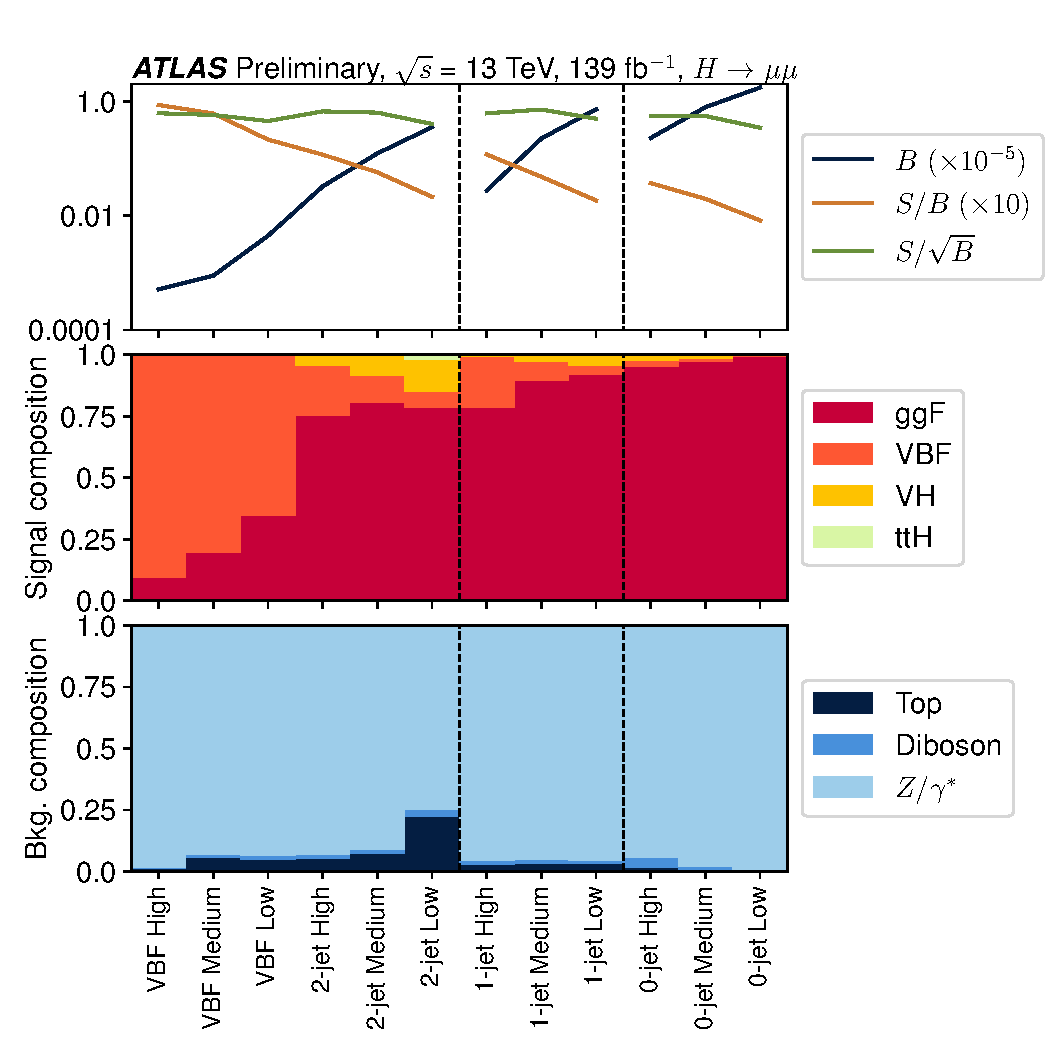
\includegraphics[width=1.0\textwidth]{figures/hmumu/cat-summary}
  \caption[Summary of $\hmumu$ analysis categories]{Summary of $\hmumu$
  analysis categories. Top panel shows the total number of background events
  in the central region, multiplied by $10^{-5}$ for visibility in blue,
  while the signal purity, multiplied by 10, is shown in orange and the
  significance proxy in green. The middle panel shows the signal
  composition of the categories, dominated by VBF events, shown in orange,
  in the VBF targetting categories, and by $\ggf$ events, shown in red,
  in all the others. VH events are shown in yellow, and $\tth$ events
  in lime. The background composition in shown in the bottom 
  panel and is dominated by DY events, shown in light blue. Diboson events
  are shown in blue, and top events in dark blue. From Ref. \cite{ATLAS-CONF-2019-028}.
  }
  \label{fig:hmumu:cat-summary}
\end{figure}

As explored in VADER4$\mu$ project, the momentum resolution of muons
is a function of their kinematics. Furthermore, the categorisation of
events in the analysis is based on a BDT classifier, which exploits
the kinematic differences between the signal and background events.
As a result, the analysis categories can have quite different
invariant mass resolutions. While this is expected, it is critical
that the modelling of dimuon mass resolution in MC simulation matches
the resolution in data in each analysis category, otherwise the
sensitivity would be over or under estimated. The validation of
the momentum calibrations, described in Section \ref{sec:muons:calibration},
is performed on the $Z$ mass peak. The validation for 0-jet High,
1-jet High, 2-jet High, and VBF High categories are shown in
Figure \ref{fig:hmumu:reso}. Bottom panels show that resolution
modelling is well within systematic uncertainties, similar results are
seen on other categories.
\begin{figure}[h!]
  \centering
  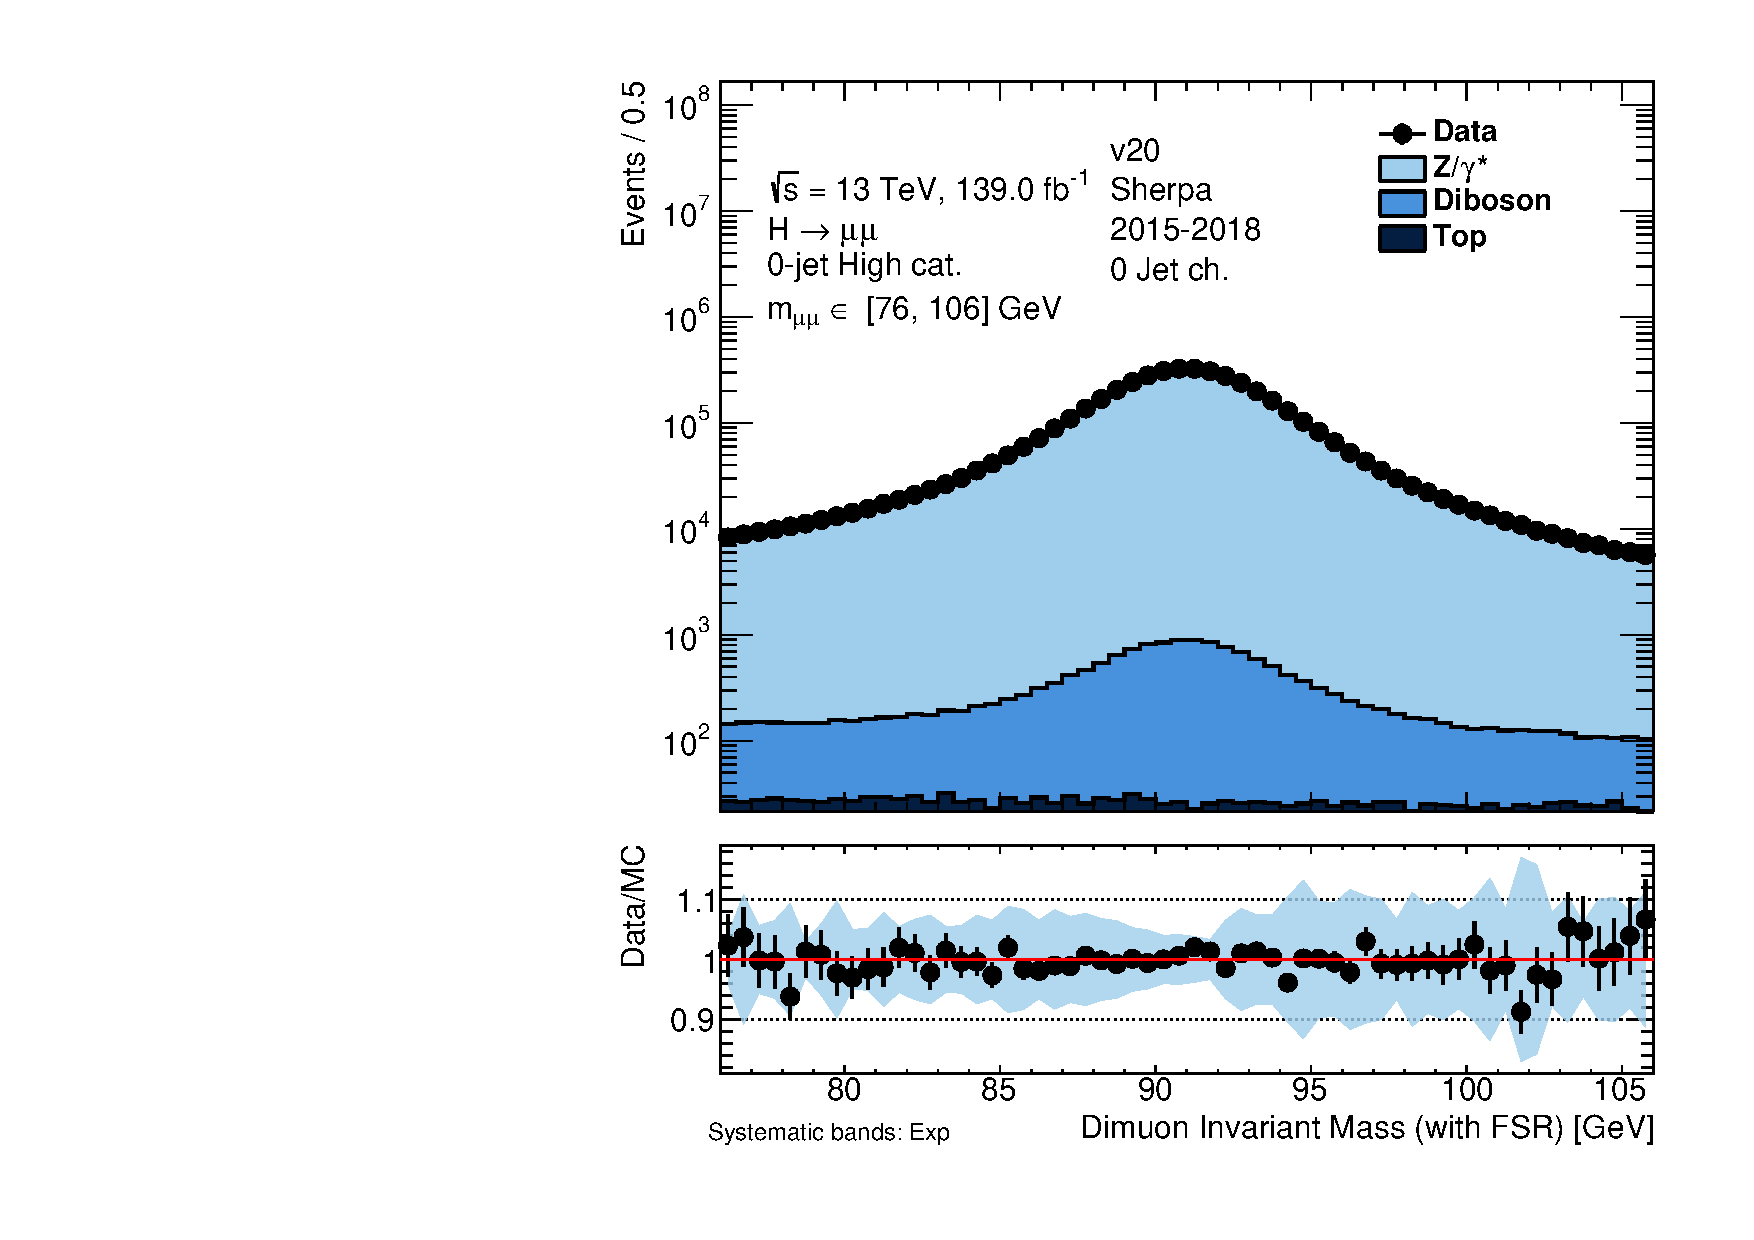
\includegraphics[width=0.49\textwidth]{figures/hmumu/reso/0jet_1}
  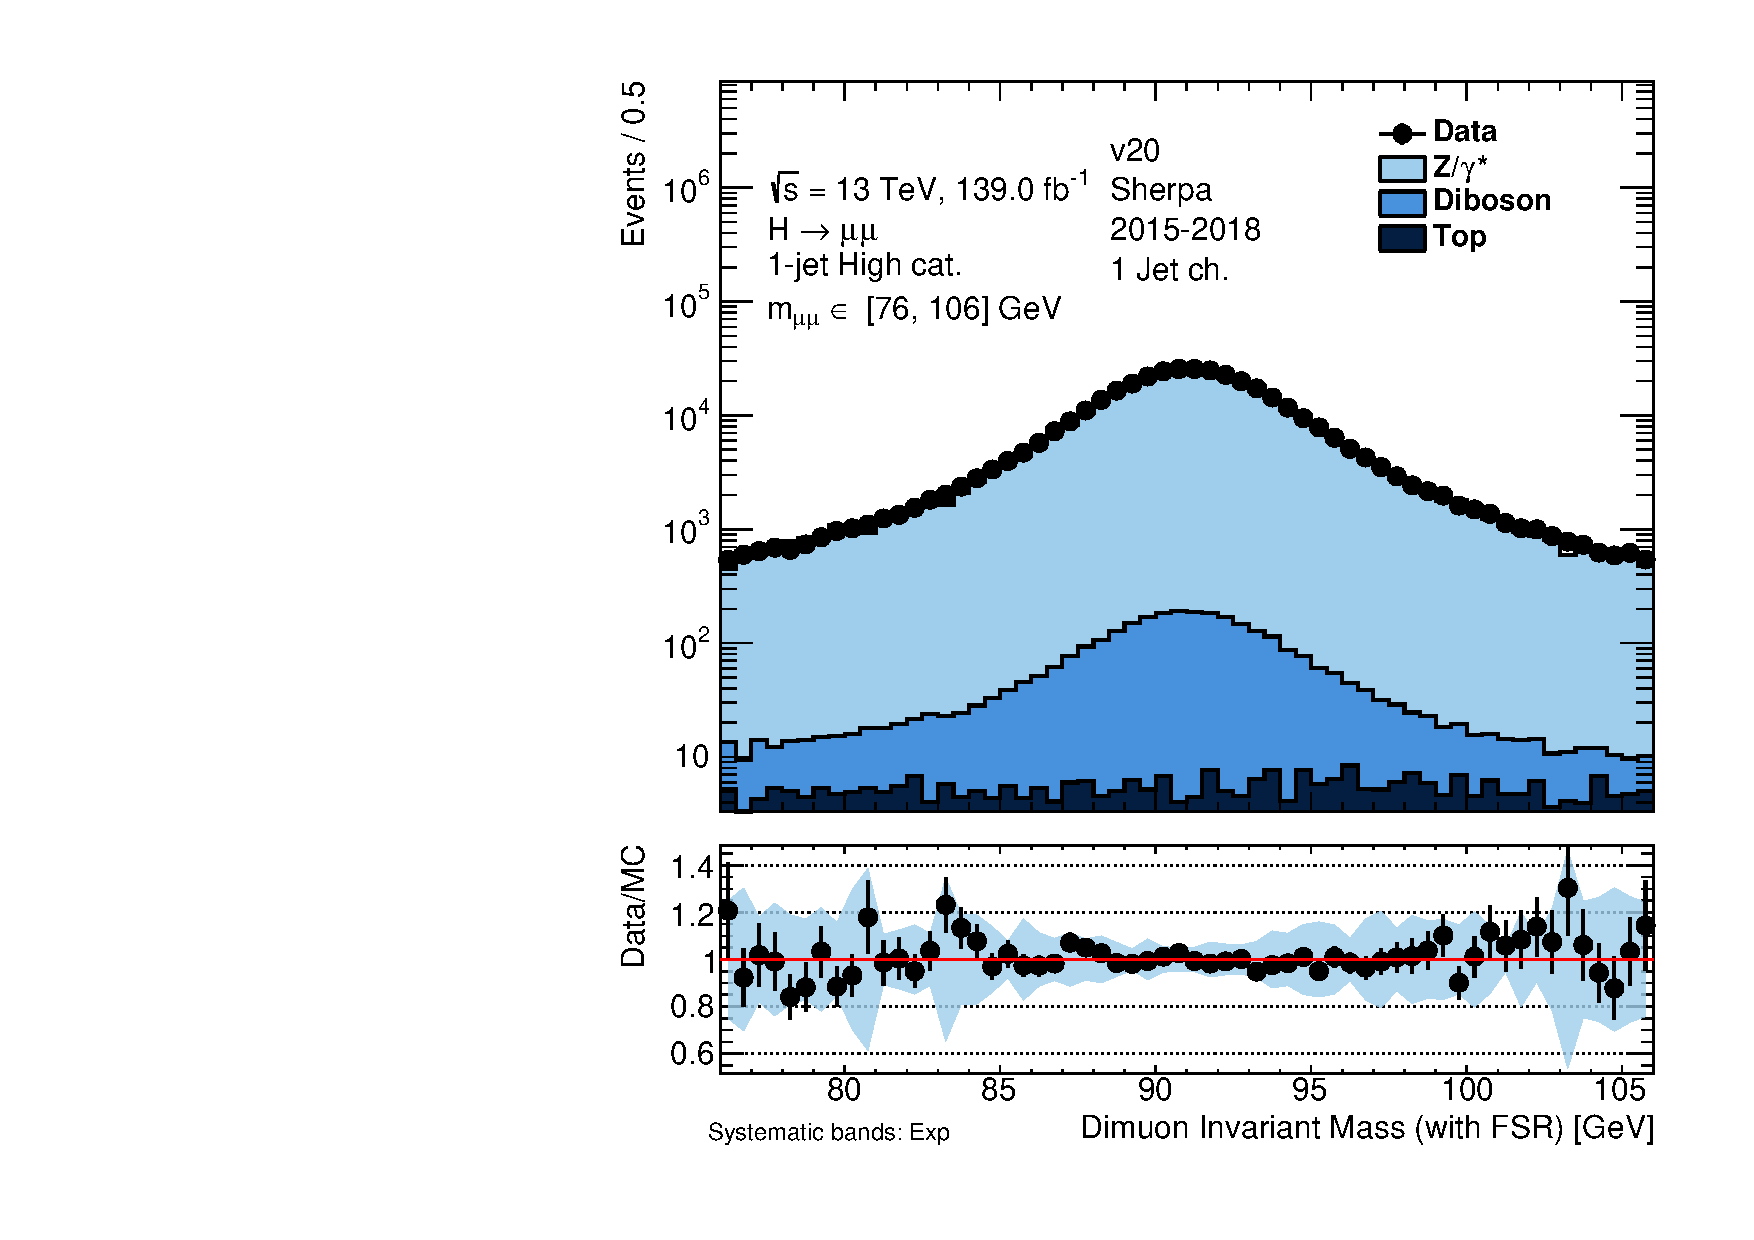
\includegraphics[width=0.49\textwidth]{figures/hmumu/reso/1jet_1}
  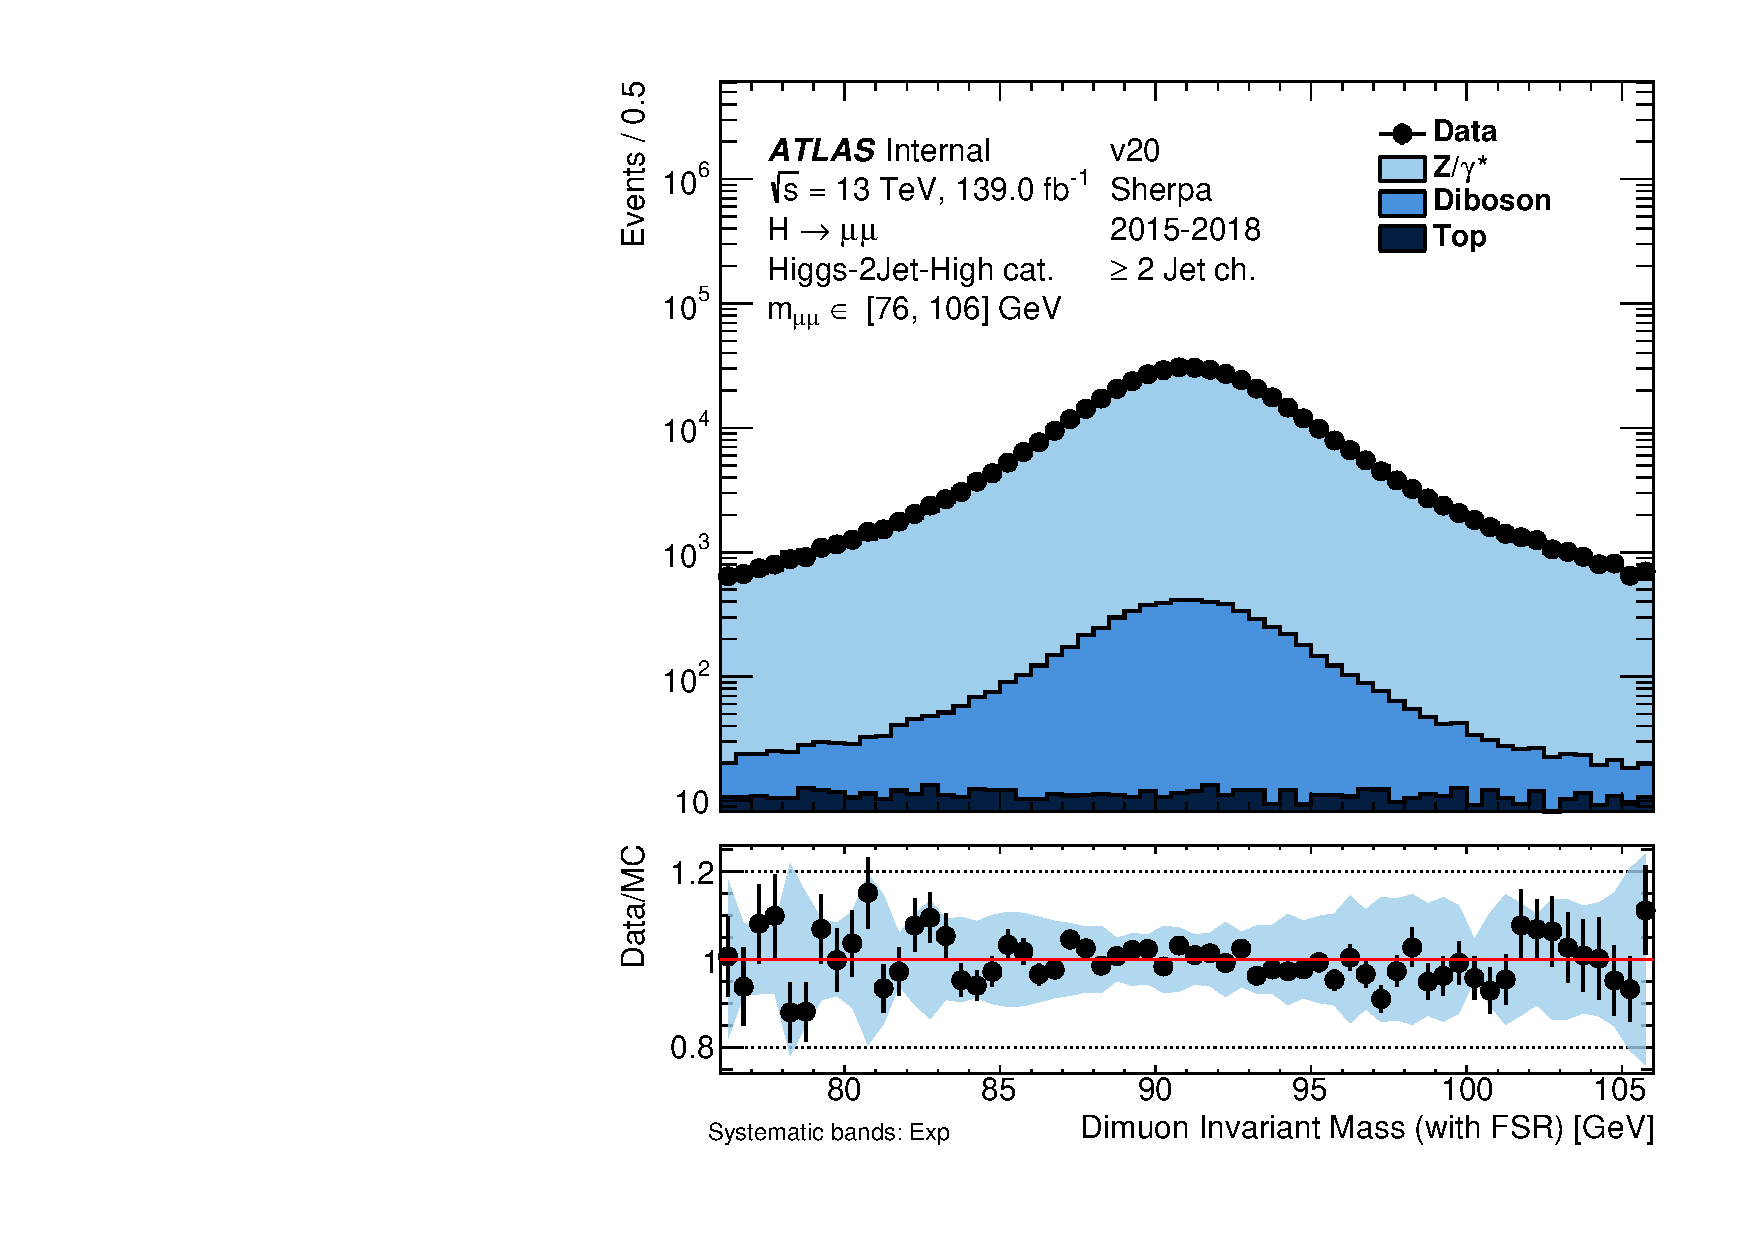
\includegraphics[width=0.49\textwidth]{figures/hmumu/reso/2jet_4}
  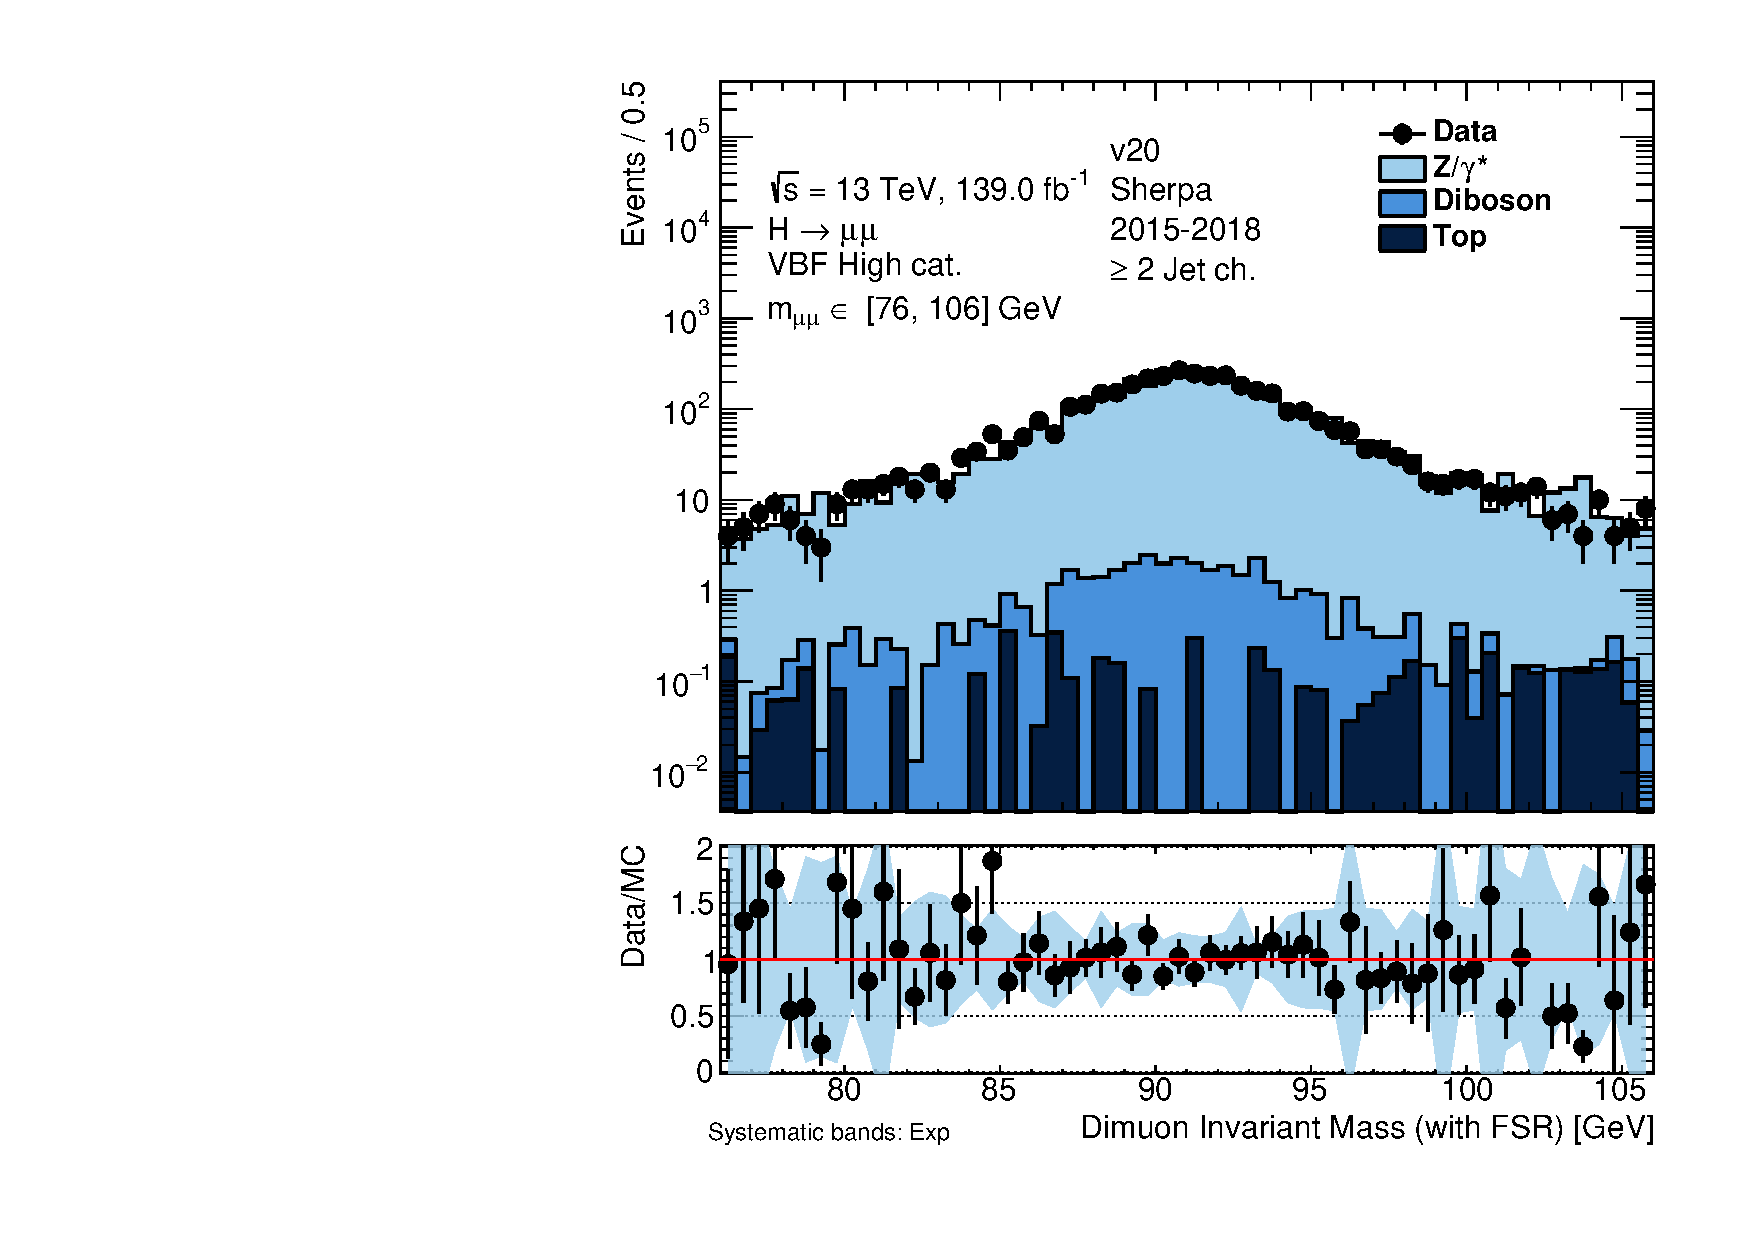
\includegraphics[width=0.49\textwidth]{figures/hmumu/reso/2jet_1}
  \caption[Mass resolution validation in analysis categories]{
  Invariant mass distribution after the FSR correction at the $Z$ peak
  for the 0-jet High, 1-jet High, 2-jet High, and VBF High
  analysis categories. Data is shown as black markers,
  Drell-Yan as light blue, diboson as blue, and top MC simulated events as
  dark blue histograms. MC simulation has been normalised to data
  for easier visual comparison. Bottom panel shows the ratio between data and
  MC simulation. Blue band represents experimental systematic
  uncertainties, while the black error bars represent combined
  statistical uncertainties on both data and MC simulation.
  }
  \label{fig:hmumu:reso}
\end{figure}

\section{Signal modelling}

The Higgs boson has a width of only 4.1 \MeV, negligible compared
to the detector resolution of a few \GeV~in this momentum range.
As a result, the signal shape is dominated by detector resolution
effect and to some extent the quality of final state radiation
recovery.

It is modelled using a double-sided Crystal-Ball (DCSB) function
\cite{Oreglia:1980cs}, which has a Gaussian core
and tails on both sides, and is defined as \cite{Aaboud:2016tru}
\begin{equation}
\newcommand{\alow}{\alpha_\text{low}}
\newcommand{\ahigh}{\alpha_\text{high}}
\newcommand{\nlow}{n_\text{low}}
\newcommand{\nhigh}{n_\text{high}}
\newcommand{\for}{\text{for }}
    \text{DCSB} = N \cdot
    \begin{cases}
      e^{-\frac{1}{2}t^2}              &  \for -\alow \leq t \leq \ahigh \\
      e^{-\frac{1}{2}\alow^2} \left[ \frac{\alow}{\nlow} \left( \frac{\nlow}{\alow} -\alow - t \right) \right]^{-\nlow}  & \for t < -\alow \\
      e^{-\frac{1}{2}\ahigh^2} \left[ \frac{\ahigh}{\nhigh} \left( \frac{\nhigh}{\ahigh} -\ahigh + t \right) \right]^{-\nhigh}  & \for t > \ahigh,
    \end{cases}
\end{equation}
where $t = (\mmumu - \mu_\text{CB}) / \sigma_\text{CB}$, $N$ is the
normalisation constant, $\mu_\text{CB}$ and $\sigma_\text{CB}$ are
the mean and sigma of the central Gaussian distribution,
$\alpha_\text{low}$ ($\alpha_\text{high}$) parametrises the
invariant mass where the function transitions to the $n_\text{low}$
($n_\text{high}$) power law on the low-mass (high-mass) side of
the spectrum.

An alternative functional form, a sum of
a Gaussian and a one-sided Crystal-Ball has been tested with similar
results. Double-sided Crystal-Ball was chosen because its
parametrisation has a single mean and width and is more stable
during the fit.

The signal shape is obtained in each category separately by fitting
the combined signal from all main production modes. An alternative
approach, fitting production modes separately and combining them
in the proportions predicted by the SM, yielded very similar results
and was abandoned for simplicity.

The detailed form of the signal shape is expected to have little
impact on the result at the search stage. Nevertheless, injection
tests were carried out, fitting the functional form to a MC simulated
spectrum. The extracted signals matched the injection withing 0.5\%,
equal to the statistical precision of the test.

The fitted values of the $\mu_\text{CB}$ parameter were between
124.5 and 124.8 \GeV, while the $\sigma_\text{CB}$ parameter varied
between 2.5 and 3.0 \GeV~between the categories. Fitted DCSB models
are shown in Figure \ref{fig:hmumu:sig-model} for the VBF High and
0-jet High categories.
\begin{figure}[h!]
  \centering
  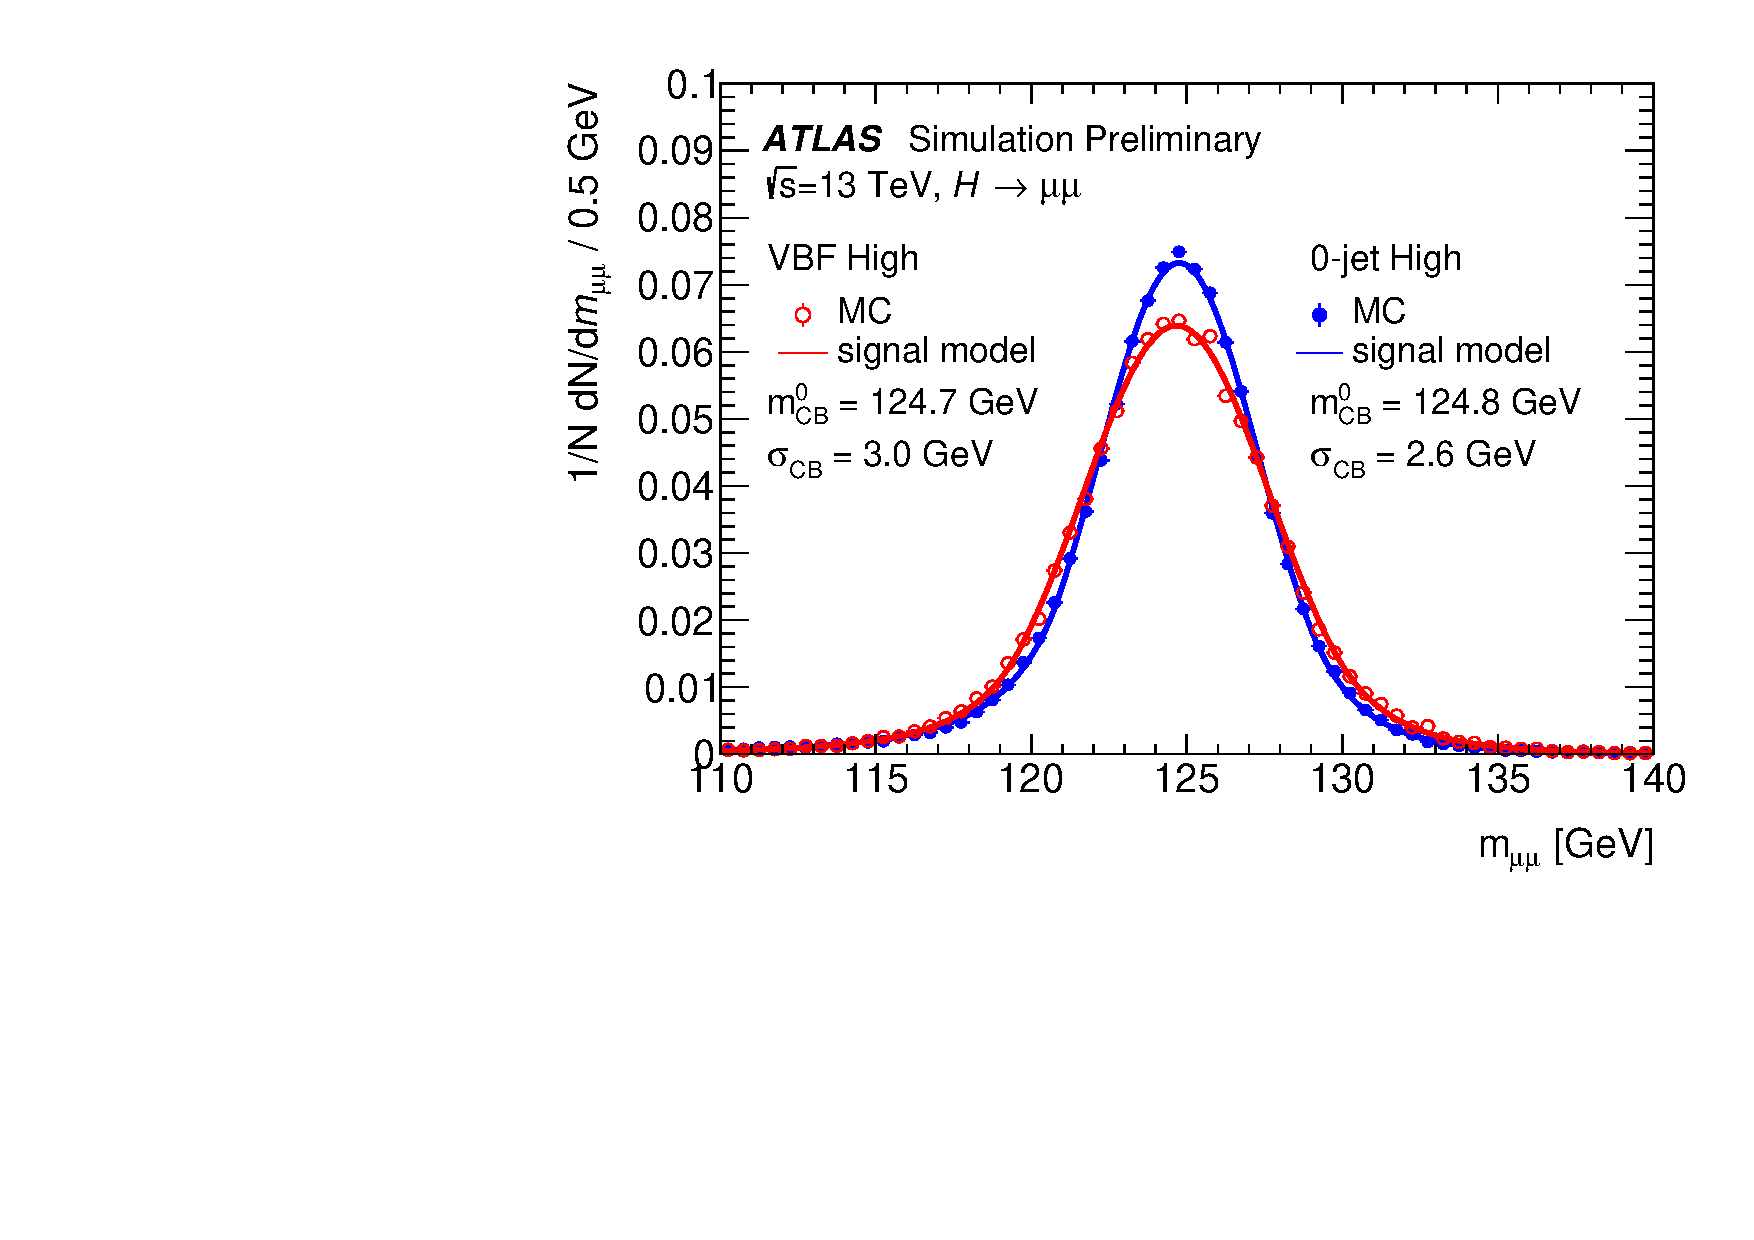
\includegraphics[width=0.8\textwidth]{figures/hmumu/sig-model}
  \caption[$\hmumu$ signal model]{
  DCSB signal model fit to the MC simulation of all Higgs production
  modes in the VBF High and 0-jet High analysis categories. VBF High
  category fit is shown as a red solid line, while the MC simulation
  is shown as empty red markers. The fit in the 0-jet High category
  is shown as a blue line, while the MC simulation is shown as solid 
  blue circles. The fitted values of $\mu_\text{CB}$ and
  $\sigma_\text{CB}$ parameters are shown on the left (right) side 
  for the VBF High (0-jet High) category. From Ref. \cite{ATLAS-CONF-2019-028}.
  }
  \label{fig:hmumu:sig-model}
\end{figure}


\section{Background modelling}

The very small signal to background ratio in the central region,
means that the modelling of the background is critical to the
success of the analysis. Since the number of background events
is much larger, a very small bias in the background model would
greatly impact the extracted signal.

The inclusive signal to background ratio is 0.2\% inclusively,
though this improves in some analysis categories. This requires
the control of the background shape to sub per mille level.

Analytical functions, motivated by the composition of the
background spectrum (dominated by DY, smaller contributions
from diboson and top), have been tried in the past but they have
struggled in particular to model the steeply falling spectrum
towards the $Z$ mass peak. In this analysis, a combination
of a rigid core and an empirical function is used instead.

The core function, common to all analysis categories and without
free parameters, models the steep part of the spectrum. The
empirical function models the differences in categories
due to selection and resolution effects, and is selected
using the custom DY dataset, described in Section \ref{sec:hmumu:customDY}.
The value of the spurious signal uncertainty is extracted
simultaneously.

\subsection{Background parametrisation}

The background model is constructed in each analysis category
separately, by multiplying a common core function with an
empirical function specific to the category
\begin{equation}
F(\mmumu) = F_\text{core}(\mmumu) \cdot F_{\text{empirical}}(\mmumu).
\end{equation}

The core function describes the inclusive DY spectrum and
is able to model the steeply falling part of the spectrum.
It is constructed from the analytic LO Drell-Yan line-shape
\cite{Aaboud:2017ffb}
\begin{equation}
F_\text{core}(\mmumu) = \sum_q \mathcal{L}_{q\bar q}(\mmumu) \cdot \sigma_{q\bar q}(\mmumu),
\end{equation}
where the sum over $q$ runs over the lightest three quarks,
$q = u, s, d$, the parton luminosity component $\mathcal{L}_{q\bar q}$
is derived using PDF4LHC15 PDF for the LO using APFEL
\cite{Bertone:2013vaa} and LHAPDF \cite{Buckley:2014ana}.
The cross-section component
$\sigma_{q\bar q}(\hat s) = \sigma_{q\bar q}(\mmumu) / (2\mmumu)$
can be written as \cite{ATLAS-CONF-2019-028}
\begin{equation}
\sigma_{q\bar q}(\hat s) = \frac{4\pi \alpha^2}{3\hat s N_c}
\left[
Q_q^2 - 2 Q_q V_\ell V_q \chi_{Z\gamma} (\hat s) +
(A_\ell^2 + V_\ell^2) (A_q^2 + V_q^2) \chi_Z(\hat s)
\right],
\end{equation}
where
\begin{align}
 \chi_{Z\gamma}(\hat s) & = \kappa \frac{\hat s (\hat s - m_Z^2)}{(\hat s - m_Z^2)^2 + \Gamma_Z^2 m_Z^2}, \\
 \chi_{Z}(\hat s)       & = \kappa^2 \frac{{\hat s}^2}{(\hat s - m_Z^2)^2 + \Gamma_Z^2 m_Z^2}, \\
 \kappa                 & = \frac{\sqrt{2}G_Fm_Z^2}{4\pi \alpha},
\end{align}
and $\hat s = \mmumu^2$, $Q_q$ is the electric charges of the quarks,
$V_f$ and $A_f$ are the vector and axial vector couplings of the fermions,
$\alpha$, $G_F$ are the electroweak couplings,
$m_Z$ and $\Gamma_Z$ are the mass and the width of the $Z$ boson \cite{Patrignani:2016xqp},
and $N_c = 3$ is the number of colour charges.



\subsection{Model selection}

procedure

selected functions and related spurious signal values

\section{Systematic uncertainties}

\subsection{Signal}

\subsection{Background}

\section{Results}



